% ==============================================================================
% Paper 3J: Mechanistic Dimensions in EDC — The Weak-Sector Brane Interface
% Journal-style synthesis (primary reading path for EDC Weak Program)
% Date: 2026-01-21
% DOI: [To be assigned upon Zenodo publication]
% ==============================================================================

\documentclass[11pt,a4paper]{article}

% ─────────────────────────────────────────────────────────────────────────────
% Required packages BEFORE shared style
% ─────────────────────────────────────────────────────────────────────────────
\usepackage{amsmath,amssymb}
\usepackage{enumitem}
\usepackage{tikz}
\usetikzlibrary{positioning,arrows.meta,shapes.geometric,calc,decorations.pathmorphing,fit,backgrounds}
\usepackage{tcolorbox}
\tcbuselibrary{skins,breakable}

% ─────────────────────────────────────────────────────────────────────────────
% Shared EDC style
% ─────────────────────────────────────────────────────────────────────────────
% edc_style.tex — Canonical EDC Paper Style for Paper 3 Series
% Version 1.0 — 2026-01-20
%
% USAGE: Include in preamble AFTER loading packages but BEFORE \begin{document}
%   % edc_style.tex — Canonical EDC Paper Style for Paper 3 Series
% Version 1.0 — 2026-01-20
%
% USAGE: Include in preamble AFTER loading packages but BEFORE \begin{document}
%   % edc_style.tex — Canonical EDC Paper Style for Paper 3 Series
% Version 1.0 — 2026-01-20
%
% USAGE: Include in preamble AFTER loading packages but BEFORE \begin{document}
%   \input{../_shared/style/edc_style}
%   \input{../_shared/style/tikz_style_edc}  % if using TikZ figures
%
% REQUIRED PACKAGES (load these in main document before \input):
%   fontspec, amsmath, amssymb, amsthm, mathtools, geometry
%   hyperref, enumitem, booktabs, array, xcolor, tcolorbox
%
% ============================================================

% ============================================================
%  EPISTEMIC TAG COLORS
% ============================================================
\definecolor{tagDer}{RGB}{0,128,0}      % Green - Derived
\definecolor{tagDc}{RGB}{0,0,200}       % Blue - Deduced/Constrained
\definecolor{tagCal}{RGB}{200,0,0}      % Red - Calibrated
\definecolor{tagP}{RGB}{128,0,128}      % Purple - Postulated
\definecolor{tagBL}{RGB}{128,128,128}   % Gray - Baseline
\definecolor{tagI}{RGB}{255,140,0}      % Orange - Identified
\definecolor{tagOpen}{RGB}{200,100,0}   % Dark orange - Open

% ============================================================
%  EPISTEMIC TAG COMMANDS
% ============================================================
% Use these to mark claims with their epistemic status
\newcommand{\tagDer}{\textcolor{tagDer}{\textbf{[Der]}}}    % Derived from axioms
\newcommand{\tagDc}{\textcolor{tagDc}{\textbf{[Dc]}}}       % Deduced/Constrained
\newcommand{\tagCal}{\textcolor{tagCal}{\textbf{[Cal]}}}    % Calibrated (fitted)
\newcommand{\tagP}{\textcolor{tagP}{\textbf{[P]}}}          % Postulated
\newcommand{\tagBL}{\textcolor{tagBL}{\textbf{[BL]}}}       % Baseline (external fact)
\newcommand{\tagI}{\textcolor{tagI}{\textbf{[I]}}}          % Identified (pattern match)
\newcommand{\tagOpen}{\textcolor{tagOpen}{\textbf{[OPEN]}}} % Open problem
\newcommand{\tagDef}{\textcolor{tagDc}{\textbf{[Def]}}}     % Definition

% ============================================================
%  THEOREM ENVIRONMENTS
% ============================================================
\newtheorem{postulate}{Postulate}
\newtheorem{definition}{Definition}[section]
\newtheorem{theorem}{Theorem}[section]
\newtheorem{lemma}[theorem]{Lemma}
\newtheorem{corollary}[theorem]{Corollary}
\newtheorem{proposition}[theorem]{Proposition}
\newtheorem{remark}{Remark}[section]

% ============================================================
%  COMMON EDC SYMBOLS
% ============================================================
% Symmetry groups
\newcommand{\Ztwo}{\mathbb{Z}_2}
\newcommand{\Zthree}{\mathbb{Z}_3}
\newcommand{\Ztri}{\mathbb{Z}_3}    % alias
\newcommand{\Zsix}{\mathbb{Z}_6}

% Geometric objects
\newcommand{\Sthree}{S^3}           % 3-sphere
\newcommand{\Stwo}{S^2}             % 2-sphere
\newcommand{\Bthree}{B^3}           % 3-ball
\newcommand{\Mfive}{\mathcal{M}_5}  % 5D manifold
\newcommand{\Bfour}{\mathcal{B}_4}  % 4D brane

% Physical quantities
\newcommand{\tension}{\tau}         % string/flux-tube tension (E/L)
\newcommand{\re}{r_e}               % electron radius

% Operators
\newcommand{\Pfrozen}{\mathcal{P}_{\mathrm{frozen}}}  % Frozen projection operator
\newcommand{\Ebrane}{\mathcal{E}_{\mathrm{brane}}}    % Brane energy store

% Bulk-brane exchange current (canonical notation from Framework v2.0)
\newcommand{\Jbb}[1]{J^{#1}_{\mathrm{bulk}\to\mathrm{brane}}}

% ============================================================
%  TCOLORBOX STYLES FOR EDC PAPERS
% ============================================================
% Cornerstone box (blue) — key claims/foundations
\tcbset{
    edcCornerstone/.style={
        colback=blue!5,
        colframe=blue!40!black,
        fonttitle=\bfseries
    }
}

% Guardrail box (gray) — epistemic warnings/constraints
\tcbset{
    edcGuardrail/.style={
        colback=gray!5!white,
        colframe=gray!60!black,
        fonttitle=\bfseries
    }
}

% PPN box (blue, lighter) — Physical Process Narrative
\tcbset{
    edcPPN/.style={
        colback=blue!5,
        colframe=blue!50!black,
        fonttitle=\bfseries
    }
}

% Canonical box (yellow/orange) — canonical definitions/glossary
\tcbset{
    edcCanonical/.style={
        colback=yellow!5,
        colframe=orange!60!black,
        fonttitle=\bfseries
    }
}

% Conceptual box (yellow/orange, lighter) — conceptual pictures
\tcbset{
    edcConcept/.style={
        colback=yellow!5,
        colframe=orange!50!black,
        fonttitle=\bfseries
    }
}

% Pathway box (purple) — energy pathways, mechanisms
\tcbset{
    edcPathway/.style={
        colback=purple!5,
        colframe=purple!40!black,
        fonttitle=\bfseries
    }
}

% Model box (green) — mechanical analogies, heuristics
\tcbset{
    edcModel/.style={
        colback=green!5,
        colframe=green!40!black,
        fonttitle=\bfseries
    }
}

% Warning box (red) — non-overclaim, limitations
\tcbset{
    edcWarning/.style={
        colback=red!5,
        colframe=red!40!black,
        fonttitle=\bfseries
    }
}

% Framework quote box (gray) — verbatim from Framework v2.0
\tcbset{
    edcFramework/.style={
        colback=gray!5!white,
        colframe=gray!60!black,
        fonttitle=\small
    }
}

% Mechanism box (teal) — mechanistic dimension principle narrative
\tcbset{
    edcMechanism/.style={
        colback=teal!5,
        colframe=teal!50!black,
        fonttitle=\bfseries,
        title={Mechanistic Dimension Note (Canon)}
    }
}

% ============================================================
%  MECHANISTIC DIMENSION HELPER MACRO
% ============================================================
% Usage: \edcMechanismNote{bulk cause}{brane process}{3D output}
%
% Example:
%   \edcMechanismNote{Junction relaxes toward Steiner minimum}%
%                    {Energy pumps into brane-layer modes, redistributes}%
%                    {Electron, antineutrino, proton emerge on 3D side}
%
\newcommand{\edcMechanismNote}[3]{%
\begin{tcolorbox}[edcMechanism]
\begin{itemize}[nosep,leftmargin=*]
    \item \textbf{5D cause (bulk):} #1
    \item \textbf{Brane-layer process:} #2
    \item \textbf{3D observation (output):} #3
\end{itemize}
\vspace{0.3em}
\footnotesize\textit{Ledger closure must hold: bulk + brane + 3D outputs conserve energy/quantum numbers.}
\end{tcolorbox}
}

% ============================================================
%  RELATED DOCUMENTS MACRO
% ============================================================
% Usage: \edcRelatedDocs{main paper title}{main DOI}{companion list}
%
% Example:
%     A: \emph{Effective Lagrangian} (\href{...}{DOI}) $\cdot$
%     B: \emph{WKB Prefactor} (\href{...}{DOI})
%   }

% NOTE: \edcRelatedDocs macro deprecated (DOI registry consolidated)
% Use consolidated Zenodo article as primary reference instead.

% ============================================================
%  DOI REGISTRY DEPRECATED
% ============================================================
% Previous individual DOIs have been deprecated.
% All EDC Weak Sector content is now consolidated into a single
% Zenodo article. See paper_3_series/19_edc_weak_sector_zenodo_article/

% ============================================================
%  PHYSICAL NARRATION RULE REMINDER
% ============================================================
% Every key equation MUST be accompanied by a physical narrative stating:
%   1. 5D cause: What changes in the bulk-core configuration?
%   2. Brane response: How does the brane absorb/redistribute energy?
%   3. 3D observable output: What do observers detect on the 3D side?
%
% This rule eliminates "numerology smell" by ensuring every formula
% has a mechanistic interpretation.

% ============================================================
%  END OF STYLE FILE
% ============================================================

%   % tikz_style_edc.tex — Reusable TikZ styles for EDC papers
% Version 1.0 — 2026-01-20
% Include via: \input{tikz_style_edc}

% ============================================================
% REQUIRED LIBRARIES (must be loaded in main document)
% ============================================================
% \usetikzlibrary{calc,angles,quotes,decorations.markings,decorations.pathmorphing,positioning}

% ============================================================
% POSITIONING DEFAULTS
% ============================================================
\tikzset{
    % Default node distances for horizontal/vertical layouts
    edc node distance/.style={node distance=1.6cm and 2.0cm},
    % Compact variant for dense diagrams
    edc compact/.style={node distance=1.2cm and 1.5cm},
    % Spread variant for clarity
    edc spread/.style={node distance=2.0cm and 2.5cm},
}

% ============================================================
% COLOR PALETTE (consistent with epistemic tags)
% ============================================================
\definecolor{edcBulk}{RGB}{220,50,50}        % Red tones for bulk/5D
\definecolor{edcBrane}{RGB}{50,150,50}       % Green tones for brane-layer
\definecolor{edcOutput}{RGB}{50,100,200}     % Blue tones for 3D outputs
\definecolor{edcNeutral}{RGB}{100,100,100}   % Gray for neutral/annotations

% ============================================================
% BOX STYLES
% ============================================================
\tikzset{
    % Generic EDC box (base style)
    edc box/.style={
        rectangle,
        draw,
        rounded corners=3pt,
        minimum width=2.2cm,
        minimum height=0.8cm,
        align=center,
        font=\small,
        inner sep=4pt,
    },
    % Bulk-core box (red family)
    bulk box/.style={
        edc box,
        fill=red!10,
        draw=edcBulk!70!black,
        text=black,
    },
    % Brane-layer box (green family)
    brane box/.style={
        edc box,
        fill=green!10,
        draw=edcBrane!70!black,
        text=black,
    },
    % 3D output box (blue family)
    output box/.style={
        edc box,
        fill=blue!10,
        draw=edcOutput!70!black,
        text=black,
    },
    % Neutral/process box
    process box/.style={
        edc box,
        fill=gray!10,
        draw=gray!60!black,
        text=black,
    },
    % Label-only box (no background)
    label box/.style={
        rectangle,
        rounded corners=2pt,
        draw=gray!40,
        fill=white,
        inner sep=2pt,
        font=\scriptsize,
    },
}

% ============================================================
% ARROW STYLES
% ============================================================
\tikzset{
    % Standard thick arrow
    edc arrow/.style={
        ->,
        >=stealth,
        thick,
    },
    % Emphasized arrow (for main flow)
    edc flow/.style={
        ->,
        >=stealth,
        very thick,
        line width=1.2pt,
    },
    % Dashed arrow (for optional/weak connections)
    edc dashed/.style={
        ->,
        >=stealth,
        thick,
        dashed,
    },
    % Double arrow (for bidirectional)
    edc bidir/.style={
        <->,
        >=stealth,
        thick,
    },
}

% ============================================================
% REGION STYLES (for background fills)
% ============================================================
\tikzset{
    % Bulk region (5D)
    bulk region/.style={
        fill=blue!8,
    },
    % Brane layer region
    brane region/.style={
        fill=yellow!25,
    },
    % Observer/3D region
    observer region/.style={
        fill=green!8,
    },
}

% ============================================================
% LABEL STYLES
% ============================================================
\tikzset{
    % Phase label (below nodes)
    phase label/.style={
        font=\scriptsize\itshape,
        text=black!70,
    },
    % Equation label (for inline math)
    eq label/.style={
        font=\scriptsize,
        fill=white,
        inner sep=1pt,
    },
    % Section annotation
    section label/.style={
        font=\footnotesize\bfseries,
        text=black,
    },
}

% ============================================================
% JUNCTION/PARTICLE STYLES
% ============================================================
\tikzset{
    % Y-junction point
    junction point/.style={
        circle,
        fill=red!60!black,
        minimum size=4pt,
        inner sep=0pt,
    },
    % Flux tube arm
    flux arm/.style={
        thick,
        blue!60!black,
    },
    % Particle dot (electron, etc.)
    particle/.style={
        circle,
        fill=black,
        minimum size=5pt,
        inner sep=0pt,
    },
    % Neutrino (smaller, gray)
    neutrino/.style={
        circle,
        fill=gray,
        minimum size=4pt,
        inner sep=0pt,
    },
}

% ============================================================
% SPRING DECORATION (for mechanical models)
% ============================================================
\tikzset{
    spring/.style={
        thick,
        decorate,
        decoration={
            coil,
            aspect=0.5,
            segment length=2mm,
            amplitude=2mm,
        },
    },
    % Wave decoration (for field modes)
    wave field/.style={
        thick,
        decorate,
        decoration={
            snake,
            amplitude=2pt,
            segment length=8pt,
        },
    },
}

% ============================================================
% BOUNDARY STYLES
% ============================================================
\tikzset{
    % Bulk-facing boundary (dashed red)
    bulk boundary/.style={
        very thick,
        red!70!black,
        dashed,
    },
    % Observer-facing boundary (solid green)
    observer boundary/.style={
        thick,
        green!50!black,
    },
    % Brane edge (orange)
    brane edge/.style={
        thick,
        orange!70!black,
    },
}

% ============================================================
% CONVENIENCE COMMANDS
% ============================================================
% Arrow label (above)
\newcommand{\arrlabel}[1]{\scriptsize #1}
% Arrow label (below)
\newcommand{\arrlabelb}[1]{\scriptsize #1}

% ============================================================
% END OF STYLE FILE
% ============================================================
  % if using TikZ figures
%
% REQUIRED PACKAGES (load these in main document before \input):
%   fontspec, amsmath, amssymb, amsthm, mathtools, geometry
%   hyperref, enumitem, booktabs, array, xcolor, tcolorbox
%
% ============================================================

% ============================================================
%  EPISTEMIC TAG COLORS
% ============================================================
\definecolor{tagDer}{RGB}{0,128,0}      % Green - Derived
\definecolor{tagDc}{RGB}{0,0,200}       % Blue - Deduced/Constrained
\definecolor{tagCal}{RGB}{200,0,0}      % Red - Calibrated
\definecolor{tagP}{RGB}{128,0,128}      % Purple - Postulated
\definecolor{tagBL}{RGB}{128,128,128}   % Gray - Baseline
\definecolor{tagI}{RGB}{255,140,0}      % Orange - Identified
\definecolor{tagOpen}{RGB}{200,100,0}   % Dark orange - Open

% ============================================================
%  EPISTEMIC TAG COMMANDS
% ============================================================
% Use these to mark claims with their epistemic status
\newcommand{\tagDer}{\textcolor{tagDer}{\textbf{[Der]}}}    % Derived from axioms
\newcommand{\tagDc}{\textcolor{tagDc}{\textbf{[Dc]}}}       % Deduced/Constrained
\newcommand{\tagCal}{\textcolor{tagCal}{\textbf{[Cal]}}}    % Calibrated (fitted)
\newcommand{\tagP}{\textcolor{tagP}{\textbf{[P]}}}          % Postulated
\newcommand{\tagBL}{\textcolor{tagBL}{\textbf{[BL]}}}       % Baseline (external fact)
\newcommand{\tagI}{\textcolor{tagI}{\textbf{[I]}}}          % Identified (pattern match)
\newcommand{\tagOpen}{\textcolor{tagOpen}{\textbf{[OPEN]}}} % Open problem
\newcommand{\tagDef}{\textcolor{tagDc}{\textbf{[Def]}}}     % Definition

% ============================================================
%  THEOREM ENVIRONMENTS
% ============================================================
\newtheorem{postulate}{Postulate}
\newtheorem{definition}{Definition}[section]
\newtheorem{theorem}{Theorem}[section]
\newtheorem{lemma}[theorem]{Lemma}
\newtheorem{corollary}[theorem]{Corollary}
\newtheorem{proposition}[theorem]{Proposition}
\newtheorem{remark}{Remark}[section]

% ============================================================
%  COMMON EDC SYMBOLS
% ============================================================
% Symmetry groups
\newcommand{\Ztwo}{\mathbb{Z}_2}
\newcommand{\Zthree}{\mathbb{Z}_3}
\newcommand{\Ztri}{\mathbb{Z}_3}    % alias
\newcommand{\Zsix}{\mathbb{Z}_6}

% Geometric objects
\newcommand{\Sthree}{S^3}           % 3-sphere
\newcommand{\Stwo}{S^2}             % 2-sphere
\newcommand{\Bthree}{B^3}           % 3-ball
\newcommand{\Mfive}{\mathcal{M}_5}  % 5D manifold
\newcommand{\Bfour}{\mathcal{B}_4}  % 4D brane

% Physical quantities
\newcommand{\tension}{\tau}         % string/flux-tube tension (E/L)
\newcommand{\re}{r_e}               % electron radius

% Operators
\newcommand{\Pfrozen}{\mathcal{P}_{\mathrm{frozen}}}  % Frozen projection operator
\newcommand{\Ebrane}{\mathcal{E}_{\mathrm{brane}}}    % Brane energy store

% Bulk-brane exchange current (canonical notation from Framework v2.0)
\newcommand{\Jbb}[1]{J^{#1}_{\mathrm{bulk}\to\mathrm{brane}}}

% ============================================================
%  TCOLORBOX STYLES FOR EDC PAPERS
% ============================================================
% Cornerstone box (blue) — key claims/foundations
\tcbset{
    edcCornerstone/.style={
        colback=blue!5,
        colframe=blue!40!black,
        fonttitle=\bfseries
    }
}

% Guardrail box (gray) — epistemic warnings/constraints
\tcbset{
    edcGuardrail/.style={
        colback=gray!5!white,
        colframe=gray!60!black,
        fonttitle=\bfseries
    }
}

% PPN box (blue, lighter) — Physical Process Narrative
\tcbset{
    edcPPN/.style={
        colback=blue!5,
        colframe=blue!50!black,
        fonttitle=\bfseries
    }
}

% Canonical box (yellow/orange) — canonical definitions/glossary
\tcbset{
    edcCanonical/.style={
        colback=yellow!5,
        colframe=orange!60!black,
        fonttitle=\bfseries
    }
}

% Conceptual box (yellow/orange, lighter) — conceptual pictures
\tcbset{
    edcConcept/.style={
        colback=yellow!5,
        colframe=orange!50!black,
        fonttitle=\bfseries
    }
}

% Pathway box (purple) — energy pathways, mechanisms
\tcbset{
    edcPathway/.style={
        colback=purple!5,
        colframe=purple!40!black,
        fonttitle=\bfseries
    }
}

% Model box (green) — mechanical analogies, heuristics
\tcbset{
    edcModel/.style={
        colback=green!5,
        colframe=green!40!black,
        fonttitle=\bfseries
    }
}

% Warning box (red) — non-overclaim, limitations
\tcbset{
    edcWarning/.style={
        colback=red!5,
        colframe=red!40!black,
        fonttitle=\bfseries
    }
}

% Framework quote box (gray) — verbatim from Framework v2.0
\tcbset{
    edcFramework/.style={
        colback=gray!5!white,
        colframe=gray!60!black,
        fonttitle=\small
    }
}

% Mechanism box (teal) — mechanistic dimension principle narrative
\tcbset{
    edcMechanism/.style={
        colback=teal!5,
        colframe=teal!50!black,
        fonttitle=\bfseries,
        title={Mechanistic Dimension Note (Canon)}
    }
}

% ============================================================
%  MECHANISTIC DIMENSION HELPER MACRO
% ============================================================
% Usage: \edcMechanismNote{bulk cause}{brane process}{3D output}
%
% Example:
%   \edcMechanismNote{Junction relaxes toward Steiner minimum}%
%                    {Energy pumps into brane-layer modes, redistributes}%
%                    {Electron, antineutrino, proton emerge on 3D side}
%
\newcommand{\edcMechanismNote}[3]{%
\begin{tcolorbox}[edcMechanism]
\begin{itemize}[nosep,leftmargin=*]
    \item \textbf{5D cause (bulk):} #1
    \item \textbf{Brane-layer process:} #2
    \item \textbf{3D observation (output):} #3
\end{itemize}
\vspace{0.3em}
\footnotesize\textit{Ledger closure must hold: bulk + brane + 3D outputs conserve energy/quantum numbers.}
\end{tcolorbox}
}

% ============================================================
%  RELATED DOCUMENTS MACRO
% ============================================================
% Usage: \edcRelatedDocs{main paper title}{main DOI}{companion list}
%
% Example:
%     A: \emph{Effective Lagrangian} (\href{...}{DOI}) $\cdot$
%     B: \emph{WKB Prefactor} (\href{...}{DOI})
%   }

% NOTE: \edcRelatedDocs macro deprecated (DOI registry consolidated)
% Use consolidated Zenodo article as primary reference instead.

% ============================================================
%  DOI REGISTRY DEPRECATED
% ============================================================
% Previous individual DOIs have been deprecated.
% All EDC Weak Sector content is now consolidated into a single
% Zenodo article. See paper_3_series/19_edc_weak_sector_zenodo_article/

% ============================================================
%  PHYSICAL NARRATION RULE REMINDER
% ============================================================
% Every key equation MUST be accompanied by a physical narrative stating:
%   1. 5D cause: What changes in the bulk-core configuration?
%   2. Brane response: How does the brane absorb/redistribute energy?
%   3. 3D observable output: What do observers detect on the 3D side?
%
% This rule eliminates "numerology smell" by ensuring every formula
% has a mechanistic interpretation.

% ============================================================
%  END OF STYLE FILE
% ============================================================

%   % tikz_style_edc.tex — Reusable TikZ styles for EDC papers
% Version 1.0 — 2026-01-20
% Include via: % tikz_style_edc.tex — Reusable TikZ styles for EDC papers
% Version 1.0 — 2026-01-20
% Include via: \input{tikz_style_edc}

% ============================================================
% REQUIRED LIBRARIES (must be loaded in main document)
% ============================================================
% \usetikzlibrary{calc,angles,quotes,decorations.markings,decorations.pathmorphing,positioning}

% ============================================================
% POSITIONING DEFAULTS
% ============================================================
\tikzset{
    % Default node distances for horizontal/vertical layouts
    edc node distance/.style={node distance=1.6cm and 2.0cm},
    % Compact variant for dense diagrams
    edc compact/.style={node distance=1.2cm and 1.5cm},
    % Spread variant for clarity
    edc spread/.style={node distance=2.0cm and 2.5cm},
}

% ============================================================
% COLOR PALETTE (consistent with epistemic tags)
% ============================================================
\definecolor{edcBulk}{RGB}{220,50,50}        % Red tones for bulk/5D
\definecolor{edcBrane}{RGB}{50,150,50}       % Green tones for brane-layer
\definecolor{edcOutput}{RGB}{50,100,200}     % Blue tones for 3D outputs
\definecolor{edcNeutral}{RGB}{100,100,100}   % Gray for neutral/annotations

% ============================================================
% BOX STYLES
% ============================================================
\tikzset{
    % Generic EDC box (base style)
    edc box/.style={
        rectangle,
        draw,
        rounded corners=3pt,
        minimum width=2.2cm,
        minimum height=0.8cm,
        align=center,
        font=\small,
        inner sep=4pt,
    },
    % Bulk-core box (red family)
    bulk box/.style={
        edc box,
        fill=red!10,
        draw=edcBulk!70!black,
        text=black,
    },
    % Brane-layer box (green family)
    brane box/.style={
        edc box,
        fill=green!10,
        draw=edcBrane!70!black,
        text=black,
    },
    % 3D output box (blue family)
    output box/.style={
        edc box,
        fill=blue!10,
        draw=edcOutput!70!black,
        text=black,
    },
    % Neutral/process box
    process box/.style={
        edc box,
        fill=gray!10,
        draw=gray!60!black,
        text=black,
    },
    % Label-only box (no background)
    label box/.style={
        rectangle,
        rounded corners=2pt,
        draw=gray!40,
        fill=white,
        inner sep=2pt,
        font=\scriptsize,
    },
}

% ============================================================
% ARROW STYLES
% ============================================================
\tikzset{
    % Standard thick arrow
    edc arrow/.style={
        ->,
        >=stealth,
        thick,
    },
    % Emphasized arrow (for main flow)
    edc flow/.style={
        ->,
        >=stealth,
        very thick,
        line width=1.2pt,
    },
    % Dashed arrow (for optional/weak connections)
    edc dashed/.style={
        ->,
        >=stealth,
        thick,
        dashed,
    },
    % Double arrow (for bidirectional)
    edc bidir/.style={
        <->,
        >=stealth,
        thick,
    },
}

% ============================================================
% REGION STYLES (for background fills)
% ============================================================
\tikzset{
    % Bulk region (5D)
    bulk region/.style={
        fill=blue!8,
    },
    % Brane layer region
    brane region/.style={
        fill=yellow!25,
    },
    % Observer/3D region
    observer region/.style={
        fill=green!8,
    },
}

% ============================================================
% LABEL STYLES
% ============================================================
\tikzset{
    % Phase label (below nodes)
    phase label/.style={
        font=\scriptsize\itshape,
        text=black!70,
    },
    % Equation label (for inline math)
    eq label/.style={
        font=\scriptsize,
        fill=white,
        inner sep=1pt,
    },
    % Section annotation
    section label/.style={
        font=\footnotesize\bfseries,
        text=black,
    },
}

% ============================================================
% JUNCTION/PARTICLE STYLES
% ============================================================
\tikzset{
    % Y-junction point
    junction point/.style={
        circle,
        fill=red!60!black,
        minimum size=4pt,
        inner sep=0pt,
    },
    % Flux tube arm
    flux arm/.style={
        thick,
        blue!60!black,
    },
    % Particle dot (electron, etc.)
    particle/.style={
        circle,
        fill=black,
        minimum size=5pt,
        inner sep=0pt,
    },
    % Neutrino (smaller, gray)
    neutrino/.style={
        circle,
        fill=gray,
        minimum size=4pt,
        inner sep=0pt,
    },
}

% ============================================================
% SPRING DECORATION (for mechanical models)
% ============================================================
\tikzset{
    spring/.style={
        thick,
        decorate,
        decoration={
            coil,
            aspect=0.5,
            segment length=2mm,
            amplitude=2mm,
        },
    },
    % Wave decoration (for field modes)
    wave field/.style={
        thick,
        decorate,
        decoration={
            snake,
            amplitude=2pt,
            segment length=8pt,
        },
    },
}

% ============================================================
% BOUNDARY STYLES
% ============================================================
\tikzset{
    % Bulk-facing boundary (dashed red)
    bulk boundary/.style={
        very thick,
        red!70!black,
        dashed,
    },
    % Observer-facing boundary (solid green)
    observer boundary/.style={
        thick,
        green!50!black,
    },
    % Brane edge (orange)
    brane edge/.style={
        thick,
        orange!70!black,
    },
}

% ============================================================
% CONVENIENCE COMMANDS
% ============================================================
% Arrow label (above)
\newcommand{\arrlabel}[1]{\scriptsize #1}
% Arrow label (below)
\newcommand{\arrlabelb}[1]{\scriptsize #1}

% ============================================================
% END OF STYLE FILE
% ============================================================


% ============================================================
% REQUIRED LIBRARIES (must be loaded in main document)
% ============================================================
% \usetikzlibrary{calc,angles,quotes,decorations.markings,decorations.pathmorphing,positioning}

% ============================================================
% POSITIONING DEFAULTS
% ============================================================
\tikzset{
    % Default node distances for horizontal/vertical layouts
    edc node distance/.style={node distance=1.6cm and 2.0cm},
    % Compact variant for dense diagrams
    edc compact/.style={node distance=1.2cm and 1.5cm},
    % Spread variant for clarity
    edc spread/.style={node distance=2.0cm and 2.5cm},
}

% ============================================================
% COLOR PALETTE (consistent with epistemic tags)
% ============================================================
\definecolor{edcBulk}{RGB}{220,50,50}        % Red tones for bulk/5D
\definecolor{edcBrane}{RGB}{50,150,50}       % Green tones for brane-layer
\definecolor{edcOutput}{RGB}{50,100,200}     % Blue tones for 3D outputs
\definecolor{edcNeutral}{RGB}{100,100,100}   % Gray for neutral/annotations

% ============================================================
% BOX STYLES
% ============================================================
\tikzset{
    % Generic EDC box (base style)
    edc box/.style={
        rectangle,
        draw,
        rounded corners=3pt,
        minimum width=2.2cm,
        minimum height=0.8cm,
        align=center,
        font=\small,
        inner sep=4pt,
    },
    % Bulk-core box (red family)
    bulk box/.style={
        edc box,
        fill=red!10,
        draw=edcBulk!70!black,
        text=black,
    },
    % Brane-layer box (green family)
    brane box/.style={
        edc box,
        fill=green!10,
        draw=edcBrane!70!black,
        text=black,
    },
    % 3D output box (blue family)
    output box/.style={
        edc box,
        fill=blue!10,
        draw=edcOutput!70!black,
        text=black,
    },
    % Neutral/process box
    process box/.style={
        edc box,
        fill=gray!10,
        draw=gray!60!black,
        text=black,
    },
    % Label-only box (no background)
    label box/.style={
        rectangle,
        rounded corners=2pt,
        draw=gray!40,
        fill=white,
        inner sep=2pt,
        font=\scriptsize,
    },
}

% ============================================================
% ARROW STYLES
% ============================================================
\tikzset{
    % Standard thick arrow
    edc arrow/.style={
        ->,
        >=stealth,
        thick,
    },
    % Emphasized arrow (for main flow)
    edc flow/.style={
        ->,
        >=stealth,
        very thick,
        line width=1.2pt,
    },
    % Dashed arrow (for optional/weak connections)
    edc dashed/.style={
        ->,
        >=stealth,
        thick,
        dashed,
    },
    % Double arrow (for bidirectional)
    edc bidir/.style={
        <->,
        >=stealth,
        thick,
    },
}

% ============================================================
% REGION STYLES (for background fills)
% ============================================================
\tikzset{
    % Bulk region (5D)
    bulk region/.style={
        fill=blue!8,
    },
    % Brane layer region
    brane region/.style={
        fill=yellow!25,
    },
    % Observer/3D region
    observer region/.style={
        fill=green!8,
    },
}

% ============================================================
% LABEL STYLES
% ============================================================
\tikzset{
    % Phase label (below nodes)
    phase label/.style={
        font=\scriptsize\itshape,
        text=black!70,
    },
    % Equation label (for inline math)
    eq label/.style={
        font=\scriptsize,
        fill=white,
        inner sep=1pt,
    },
    % Section annotation
    section label/.style={
        font=\footnotesize\bfseries,
        text=black,
    },
}

% ============================================================
% JUNCTION/PARTICLE STYLES
% ============================================================
\tikzset{
    % Y-junction point
    junction point/.style={
        circle,
        fill=red!60!black,
        minimum size=4pt,
        inner sep=0pt,
    },
    % Flux tube arm
    flux arm/.style={
        thick,
        blue!60!black,
    },
    % Particle dot (electron, etc.)
    particle/.style={
        circle,
        fill=black,
        minimum size=5pt,
        inner sep=0pt,
    },
    % Neutrino (smaller, gray)
    neutrino/.style={
        circle,
        fill=gray,
        minimum size=4pt,
        inner sep=0pt,
    },
}

% ============================================================
% SPRING DECORATION (for mechanical models)
% ============================================================
\tikzset{
    spring/.style={
        thick,
        decorate,
        decoration={
            coil,
            aspect=0.5,
            segment length=2mm,
            amplitude=2mm,
        },
    },
    % Wave decoration (for field modes)
    wave field/.style={
        thick,
        decorate,
        decoration={
            snake,
            amplitude=2pt,
            segment length=8pt,
        },
    },
}

% ============================================================
% BOUNDARY STYLES
% ============================================================
\tikzset{
    % Bulk-facing boundary (dashed red)
    bulk boundary/.style={
        very thick,
        red!70!black,
        dashed,
    },
    % Observer-facing boundary (solid green)
    observer boundary/.style={
        thick,
        green!50!black,
    },
    % Brane edge (orange)
    brane edge/.style={
        thick,
        orange!70!black,
    },
}

% ============================================================
% CONVENIENCE COMMANDS
% ============================================================
% Arrow label (above)
\newcommand{\arrlabel}[1]{\scriptsize #1}
% Arrow label (below)
\newcommand{\arrlabelb}[1]{\scriptsize #1}

% ============================================================
% END OF STYLE FILE
% ============================================================
  % if using TikZ figures
%
% REQUIRED PACKAGES (load these in main document before \input):
%   fontspec, amsmath, amssymb, amsthm, mathtools, geometry
%   hyperref, enumitem, booktabs, array, xcolor, tcolorbox
%
% ============================================================

% ============================================================
%  EPISTEMIC TAG COLORS
% ============================================================
\definecolor{tagDer}{RGB}{0,128,0}      % Green - Derived
\definecolor{tagDc}{RGB}{0,0,200}       % Blue - Deduced/Constrained
\definecolor{tagCal}{RGB}{200,0,0}      % Red - Calibrated
\definecolor{tagP}{RGB}{128,0,128}      % Purple - Postulated
\definecolor{tagBL}{RGB}{128,128,128}   % Gray - Baseline
\definecolor{tagI}{RGB}{255,140,0}      % Orange - Identified
\definecolor{tagOpen}{RGB}{200,100,0}   % Dark orange - Open

% ============================================================
%  EPISTEMIC TAG COMMANDS
% ============================================================
% Use these to mark claims with their epistemic status
\newcommand{\tagDer}{\textcolor{tagDer}{\textbf{[Der]}}}    % Derived from axioms
\newcommand{\tagDc}{\textcolor{tagDc}{\textbf{[Dc]}}}       % Deduced/Constrained
\newcommand{\tagCal}{\textcolor{tagCal}{\textbf{[Cal]}}}    % Calibrated (fitted)
\newcommand{\tagP}{\textcolor{tagP}{\textbf{[P]}}}          % Postulated
\newcommand{\tagBL}{\textcolor{tagBL}{\textbf{[BL]}}}       % Baseline (external fact)
\newcommand{\tagI}{\textcolor{tagI}{\textbf{[I]}}}          % Identified (pattern match)
\newcommand{\tagOpen}{\textcolor{tagOpen}{\textbf{[OPEN]}}} % Open problem
\newcommand{\tagDef}{\textcolor{tagDc}{\textbf{[Def]}}}     % Definition

% ============================================================
%  THEOREM ENVIRONMENTS
% ============================================================
\newtheorem{postulate}{Postulate}
\newtheorem{definition}{Definition}[section]
\newtheorem{theorem}{Theorem}[section]
\newtheorem{lemma}[theorem]{Lemma}
\newtheorem{corollary}[theorem]{Corollary}
\newtheorem{proposition}[theorem]{Proposition}
\newtheorem{remark}{Remark}[section]

% ============================================================
%  COMMON EDC SYMBOLS
% ============================================================
% Symmetry groups
\newcommand{\Ztwo}{\mathbb{Z}_2}
\newcommand{\Zthree}{\mathbb{Z}_3}
\newcommand{\Ztri}{\mathbb{Z}_3}    % alias
\newcommand{\Zsix}{\mathbb{Z}_6}

% Geometric objects
\newcommand{\Sthree}{S^3}           % 3-sphere
\newcommand{\Stwo}{S^2}             % 2-sphere
\newcommand{\Bthree}{B^3}           % 3-ball
\newcommand{\Mfive}{\mathcal{M}_5}  % 5D manifold
\newcommand{\Bfour}{\mathcal{B}_4}  % 4D brane

% Physical quantities
\newcommand{\tension}{\tau}         % string/flux-tube tension (E/L)
\newcommand{\re}{r_e}               % electron radius

% Operators
\newcommand{\Pfrozen}{\mathcal{P}_{\mathrm{frozen}}}  % Frozen projection operator
\newcommand{\Ebrane}{\mathcal{E}_{\mathrm{brane}}}    % Brane energy store

% Bulk-brane exchange current (canonical notation from Framework v2.0)
\newcommand{\Jbb}[1]{J^{#1}_{\mathrm{bulk}\to\mathrm{brane}}}

% ============================================================
%  TCOLORBOX STYLES FOR EDC PAPERS
% ============================================================
% Cornerstone box (blue) — key claims/foundations
\tcbset{
    edcCornerstone/.style={
        colback=blue!5,
        colframe=blue!40!black,
        fonttitle=\bfseries
    }
}

% Guardrail box (gray) — epistemic warnings/constraints
\tcbset{
    edcGuardrail/.style={
        colback=gray!5!white,
        colframe=gray!60!black,
        fonttitle=\bfseries
    }
}

% PPN box (blue, lighter) — Physical Process Narrative
\tcbset{
    edcPPN/.style={
        colback=blue!5,
        colframe=blue!50!black,
        fonttitle=\bfseries
    }
}

% Canonical box (yellow/orange) — canonical definitions/glossary
\tcbset{
    edcCanonical/.style={
        colback=yellow!5,
        colframe=orange!60!black,
        fonttitle=\bfseries
    }
}

% Conceptual box (yellow/orange, lighter) — conceptual pictures
\tcbset{
    edcConcept/.style={
        colback=yellow!5,
        colframe=orange!50!black,
        fonttitle=\bfseries
    }
}

% Pathway box (purple) — energy pathways, mechanisms
\tcbset{
    edcPathway/.style={
        colback=purple!5,
        colframe=purple!40!black,
        fonttitle=\bfseries
    }
}

% Model box (green) — mechanical analogies, heuristics
\tcbset{
    edcModel/.style={
        colback=green!5,
        colframe=green!40!black,
        fonttitle=\bfseries
    }
}

% Warning box (red) — non-overclaim, limitations
\tcbset{
    edcWarning/.style={
        colback=red!5,
        colframe=red!40!black,
        fonttitle=\bfseries
    }
}

% Framework quote box (gray) — verbatim from Framework v2.0
\tcbset{
    edcFramework/.style={
        colback=gray!5!white,
        colframe=gray!60!black,
        fonttitle=\small
    }
}

% Mechanism box (teal) — mechanistic dimension principle narrative
\tcbset{
    edcMechanism/.style={
        colback=teal!5,
        colframe=teal!50!black,
        fonttitle=\bfseries,
        title={Mechanistic Dimension Note (Canon)}
    }
}

% ============================================================
%  MECHANISTIC DIMENSION HELPER MACRO
% ============================================================
% Usage: \edcMechanismNote{bulk cause}{brane process}{3D output}
%
% Example:
%   \edcMechanismNote{Junction relaxes toward Steiner minimum}%
%                    {Energy pumps into brane-layer modes, redistributes}%
%                    {Electron, antineutrino, proton emerge on 3D side}
%
\newcommand{\edcMechanismNote}[3]{%
\begin{tcolorbox}[edcMechanism]
\begin{itemize}[nosep,leftmargin=*]
    \item \textbf{5D cause (bulk):} #1
    \item \textbf{Brane-layer process:} #2
    \item \textbf{3D observation (output):} #3
\end{itemize}
\vspace{0.3em}
\footnotesize\textit{Ledger closure must hold: bulk + brane + 3D outputs conserve energy/quantum numbers.}
\end{tcolorbox}
}

% ============================================================
%  RELATED DOCUMENTS MACRO
% ============================================================
% Usage: \edcRelatedDocs{main paper title}{main DOI}{companion list}
%
% Example:
%     A: \emph{Effective Lagrangian} (\href{...}{DOI}) $\cdot$
%     B: \emph{WKB Prefactor} (\href{...}{DOI})
%   }

% NOTE: \edcRelatedDocs macro deprecated (DOI registry consolidated)
% Use consolidated Zenodo article as primary reference instead.

% ============================================================
%  DOI REGISTRY DEPRECATED
% ============================================================
% Previous individual DOIs have been deprecated.
% All EDC Weak Sector content is now consolidated into a single
% Zenodo article. See paper_3_series/19_edc_weak_sector_zenodo_article/

% ============================================================
%  PHYSICAL NARRATION RULE REMINDER
% ============================================================
% Every key equation MUST be accompanied by a physical narrative stating:
%   1. 5D cause: What changes in the bulk-core configuration?
%   2. Brane response: How does the brane absorb/redistribute energy?
%   3. 3D observable output: What do observers detect on the 3D side?
%
% This rule eliminates "numerology smell" by ensuring every formula
% has a mechanistic interpretation.

% ============================================================
%  END OF STYLE FILE
% ============================================================

% tikz_style_edc.tex — Reusable TikZ styles for EDC papers
% Version 1.0 — 2026-01-20
% Include via: % tikz_style_edc.tex — Reusable TikZ styles for EDC papers
% Version 1.0 — 2026-01-20
% Include via: % tikz_style_edc.tex — Reusable TikZ styles for EDC papers
% Version 1.0 — 2026-01-20
% Include via: \input{tikz_style_edc}

% ============================================================
% REQUIRED LIBRARIES (must be loaded in main document)
% ============================================================
% \usetikzlibrary{calc,angles,quotes,decorations.markings,decorations.pathmorphing,positioning}

% ============================================================
% POSITIONING DEFAULTS
% ============================================================
\tikzset{
    % Default node distances for horizontal/vertical layouts
    edc node distance/.style={node distance=1.6cm and 2.0cm},
    % Compact variant for dense diagrams
    edc compact/.style={node distance=1.2cm and 1.5cm},
    % Spread variant for clarity
    edc spread/.style={node distance=2.0cm and 2.5cm},
}

% ============================================================
% COLOR PALETTE (consistent with epistemic tags)
% ============================================================
\definecolor{edcBulk}{RGB}{220,50,50}        % Red tones for bulk/5D
\definecolor{edcBrane}{RGB}{50,150,50}       % Green tones for brane-layer
\definecolor{edcOutput}{RGB}{50,100,200}     % Blue tones for 3D outputs
\definecolor{edcNeutral}{RGB}{100,100,100}   % Gray for neutral/annotations

% ============================================================
% BOX STYLES
% ============================================================
\tikzset{
    % Generic EDC box (base style)
    edc box/.style={
        rectangle,
        draw,
        rounded corners=3pt,
        minimum width=2.2cm,
        minimum height=0.8cm,
        align=center,
        font=\small,
        inner sep=4pt,
    },
    % Bulk-core box (red family)
    bulk box/.style={
        edc box,
        fill=red!10,
        draw=edcBulk!70!black,
        text=black,
    },
    % Brane-layer box (green family)
    brane box/.style={
        edc box,
        fill=green!10,
        draw=edcBrane!70!black,
        text=black,
    },
    % 3D output box (blue family)
    output box/.style={
        edc box,
        fill=blue!10,
        draw=edcOutput!70!black,
        text=black,
    },
    % Neutral/process box
    process box/.style={
        edc box,
        fill=gray!10,
        draw=gray!60!black,
        text=black,
    },
    % Label-only box (no background)
    label box/.style={
        rectangle,
        rounded corners=2pt,
        draw=gray!40,
        fill=white,
        inner sep=2pt,
        font=\scriptsize,
    },
}

% ============================================================
% ARROW STYLES
% ============================================================
\tikzset{
    % Standard thick arrow
    edc arrow/.style={
        ->,
        >=stealth,
        thick,
    },
    % Emphasized arrow (for main flow)
    edc flow/.style={
        ->,
        >=stealth,
        very thick,
        line width=1.2pt,
    },
    % Dashed arrow (for optional/weak connections)
    edc dashed/.style={
        ->,
        >=stealth,
        thick,
        dashed,
    },
    % Double arrow (for bidirectional)
    edc bidir/.style={
        <->,
        >=stealth,
        thick,
    },
}

% ============================================================
% REGION STYLES (for background fills)
% ============================================================
\tikzset{
    % Bulk region (5D)
    bulk region/.style={
        fill=blue!8,
    },
    % Brane layer region
    brane region/.style={
        fill=yellow!25,
    },
    % Observer/3D region
    observer region/.style={
        fill=green!8,
    },
}

% ============================================================
% LABEL STYLES
% ============================================================
\tikzset{
    % Phase label (below nodes)
    phase label/.style={
        font=\scriptsize\itshape,
        text=black!70,
    },
    % Equation label (for inline math)
    eq label/.style={
        font=\scriptsize,
        fill=white,
        inner sep=1pt,
    },
    % Section annotation
    section label/.style={
        font=\footnotesize\bfseries,
        text=black,
    },
}

% ============================================================
% JUNCTION/PARTICLE STYLES
% ============================================================
\tikzset{
    % Y-junction point
    junction point/.style={
        circle,
        fill=red!60!black,
        minimum size=4pt,
        inner sep=0pt,
    },
    % Flux tube arm
    flux arm/.style={
        thick,
        blue!60!black,
    },
    % Particle dot (electron, etc.)
    particle/.style={
        circle,
        fill=black,
        minimum size=5pt,
        inner sep=0pt,
    },
    % Neutrino (smaller, gray)
    neutrino/.style={
        circle,
        fill=gray,
        minimum size=4pt,
        inner sep=0pt,
    },
}

% ============================================================
% SPRING DECORATION (for mechanical models)
% ============================================================
\tikzset{
    spring/.style={
        thick,
        decorate,
        decoration={
            coil,
            aspect=0.5,
            segment length=2mm,
            amplitude=2mm,
        },
    },
    % Wave decoration (for field modes)
    wave field/.style={
        thick,
        decorate,
        decoration={
            snake,
            amplitude=2pt,
            segment length=8pt,
        },
    },
}

% ============================================================
% BOUNDARY STYLES
% ============================================================
\tikzset{
    % Bulk-facing boundary (dashed red)
    bulk boundary/.style={
        very thick,
        red!70!black,
        dashed,
    },
    % Observer-facing boundary (solid green)
    observer boundary/.style={
        thick,
        green!50!black,
    },
    % Brane edge (orange)
    brane edge/.style={
        thick,
        orange!70!black,
    },
}

% ============================================================
% CONVENIENCE COMMANDS
% ============================================================
% Arrow label (above)
\newcommand{\arrlabel}[1]{\scriptsize #1}
% Arrow label (below)
\newcommand{\arrlabelb}[1]{\scriptsize #1}

% ============================================================
% END OF STYLE FILE
% ============================================================


% ============================================================
% REQUIRED LIBRARIES (must be loaded in main document)
% ============================================================
% \usetikzlibrary{calc,angles,quotes,decorations.markings,decorations.pathmorphing,positioning}

% ============================================================
% POSITIONING DEFAULTS
% ============================================================
\tikzset{
    % Default node distances for horizontal/vertical layouts
    edc node distance/.style={node distance=1.6cm and 2.0cm},
    % Compact variant for dense diagrams
    edc compact/.style={node distance=1.2cm and 1.5cm},
    % Spread variant for clarity
    edc spread/.style={node distance=2.0cm and 2.5cm},
}

% ============================================================
% COLOR PALETTE (consistent with epistemic tags)
% ============================================================
\definecolor{edcBulk}{RGB}{220,50,50}        % Red tones for bulk/5D
\definecolor{edcBrane}{RGB}{50,150,50}       % Green tones for brane-layer
\definecolor{edcOutput}{RGB}{50,100,200}     % Blue tones for 3D outputs
\definecolor{edcNeutral}{RGB}{100,100,100}   % Gray for neutral/annotations

% ============================================================
% BOX STYLES
% ============================================================
\tikzset{
    % Generic EDC box (base style)
    edc box/.style={
        rectangle,
        draw,
        rounded corners=3pt,
        minimum width=2.2cm,
        minimum height=0.8cm,
        align=center,
        font=\small,
        inner sep=4pt,
    },
    % Bulk-core box (red family)
    bulk box/.style={
        edc box,
        fill=red!10,
        draw=edcBulk!70!black,
        text=black,
    },
    % Brane-layer box (green family)
    brane box/.style={
        edc box,
        fill=green!10,
        draw=edcBrane!70!black,
        text=black,
    },
    % 3D output box (blue family)
    output box/.style={
        edc box,
        fill=blue!10,
        draw=edcOutput!70!black,
        text=black,
    },
    % Neutral/process box
    process box/.style={
        edc box,
        fill=gray!10,
        draw=gray!60!black,
        text=black,
    },
    % Label-only box (no background)
    label box/.style={
        rectangle,
        rounded corners=2pt,
        draw=gray!40,
        fill=white,
        inner sep=2pt,
        font=\scriptsize,
    },
}

% ============================================================
% ARROW STYLES
% ============================================================
\tikzset{
    % Standard thick arrow
    edc arrow/.style={
        ->,
        >=stealth,
        thick,
    },
    % Emphasized arrow (for main flow)
    edc flow/.style={
        ->,
        >=stealth,
        very thick,
        line width=1.2pt,
    },
    % Dashed arrow (for optional/weak connections)
    edc dashed/.style={
        ->,
        >=stealth,
        thick,
        dashed,
    },
    % Double arrow (for bidirectional)
    edc bidir/.style={
        <->,
        >=stealth,
        thick,
    },
}

% ============================================================
% REGION STYLES (for background fills)
% ============================================================
\tikzset{
    % Bulk region (5D)
    bulk region/.style={
        fill=blue!8,
    },
    % Brane layer region
    brane region/.style={
        fill=yellow!25,
    },
    % Observer/3D region
    observer region/.style={
        fill=green!8,
    },
}

% ============================================================
% LABEL STYLES
% ============================================================
\tikzset{
    % Phase label (below nodes)
    phase label/.style={
        font=\scriptsize\itshape,
        text=black!70,
    },
    % Equation label (for inline math)
    eq label/.style={
        font=\scriptsize,
        fill=white,
        inner sep=1pt,
    },
    % Section annotation
    section label/.style={
        font=\footnotesize\bfseries,
        text=black,
    },
}

% ============================================================
% JUNCTION/PARTICLE STYLES
% ============================================================
\tikzset{
    % Y-junction point
    junction point/.style={
        circle,
        fill=red!60!black,
        minimum size=4pt,
        inner sep=0pt,
    },
    % Flux tube arm
    flux arm/.style={
        thick,
        blue!60!black,
    },
    % Particle dot (electron, etc.)
    particle/.style={
        circle,
        fill=black,
        minimum size=5pt,
        inner sep=0pt,
    },
    % Neutrino (smaller, gray)
    neutrino/.style={
        circle,
        fill=gray,
        minimum size=4pt,
        inner sep=0pt,
    },
}

% ============================================================
% SPRING DECORATION (for mechanical models)
% ============================================================
\tikzset{
    spring/.style={
        thick,
        decorate,
        decoration={
            coil,
            aspect=0.5,
            segment length=2mm,
            amplitude=2mm,
        },
    },
    % Wave decoration (for field modes)
    wave field/.style={
        thick,
        decorate,
        decoration={
            snake,
            amplitude=2pt,
            segment length=8pt,
        },
    },
}

% ============================================================
% BOUNDARY STYLES
% ============================================================
\tikzset{
    % Bulk-facing boundary (dashed red)
    bulk boundary/.style={
        very thick,
        red!70!black,
        dashed,
    },
    % Observer-facing boundary (solid green)
    observer boundary/.style={
        thick,
        green!50!black,
    },
    % Brane edge (orange)
    brane edge/.style={
        thick,
        orange!70!black,
    },
}

% ============================================================
% CONVENIENCE COMMANDS
% ============================================================
% Arrow label (above)
\newcommand{\arrlabel}[1]{\scriptsize #1}
% Arrow label (below)
\newcommand{\arrlabelb}[1]{\scriptsize #1}

% ============================================================
% END OF STYLE FILE
% ============================================================


% ============================================================
% REQUIRED LIBRARIES (must be loaded in main document)
% ============================================================
% \usetikzlibrary{calc,angles,quotes,decorations.markings,decorations.pathmorphing,positioning}

% ============================================================
% POSITIONING DEFAULTS
% ============================================================
\tikzset{
    % Default node distances for horizontal/vertical layouts
    edc node distance/.style={node distance=1.6cm and 2.0cm},
    % Compact variant for dense diagrams
    edc compact/.style={node distance=1.2cm and 1.5cm},
    % Spread variant for clarity
    edc spread/.style={node distance=2.0cm and 2.5cm},
}

% ============================================================
% COLOR PALETTE (consistent with epistemic tags)
% ============================================================
\definecolor{edcBulk}{RGB}{220,50,50}        % Red tones for bulk/5D
\definecolor{edcBrane}{RGB}{50,150,50}       % Green tones for brane-layer
\definecolor{edcOutput}{RGB}{50,100,200}     % Blue tones for 3D outputs
\definecolor{edcNeutral}{RGB}{100,100,100}   % Gray for neutral/annotations

% ============================================================
% BOX STYLES
% ============================================================
\tikzset{
    % Generic EDC box (base style)
    edc box/.style={
        rectangle,
        draw,
        rounded corners=3pt,
        minimum width=2.2cm,
        minimum height=0.8cm,
        align=center,
        font=\small,
        inner sep=4pt,
    },
    % Bulk-core box (red family)
    bulk box/.style={
        edc box,
        fill=red!10,
        draw=edcBulk!70!black,
        text=black,
    },
    % Brane-layer box (green family)
    brane box/.style={
        edc box,
        fill=green!10,
        draw=edcBrane!70!black,
        text=black,
    },
    % 3D output box (blue family)
    output box/.style={
        edc box,
        fill=blue!10,
        draw=edcOutput!70!black,
        text=black,
    },
    % Neutral/process box
    process box/.style={
        edc box,
        fill=gray!10,
        draw=gray!60!black,
        text=black,
    },
    % Label-only box (no background)
    label box/.style={
        rectangle,
        rounded corners=2pt,
        draw=gray!40,
        fill=white,
        inner sep=2pt,
        font=\scriptsize,
    },
}

% ============================================================
% ARROW STYLES
% ============================================================
\tikzset{
    % Standard thick arrow
    edc arrow/.style={
        ->,
        >=stealth,
        thick,
    },
    % Emphasized arrow (for main flow)
    edc flow/.style={
        ->,
        >=stealth,
        very thick,
        line width=1.2pt,
    },
    % Dashed arrow (for optional/weak connections)
    edc dashed/.style={
        ->,
        >=stealth,
        thick,
        dashed,
    },
    % Double arrow (for bidirectional)
    edc bidir/.style={
        <->,
        >=stealth,
        thick,
    },
}

% ============================================================
% REGION STYLES (for background fills)
% ============================================================
\tikzset{
    % Bulk region (5D)
    bulk region/.style={
        fill=blue!8,
    },
    % Brane layer region
    brane region/.style={
        fill=yellow!25,
    },
    % Observer/3D region
    observer region/.style={
        fill=green!8,
    },
}

% ============================================================
% LABEL STYLES
% ============================================================
\tikzset{
    % Phase label (below nodes)
    phase label/.style={
        font=\scriptsize\itshape,
        text=black!70,
    },
    % Equation label (for inline math)
    eq label/.style={
        font=\scriptsize,
        fill=white,
        inner sep=1pt,
    },
    % Section annotation
    section label/.style={
        font=\footnotesize\bfseries,
        text=black,
    },
}

% ============================================================
% JUNCTION/PARTICLE STYLES
% ============================================================
\tikzset{
    % Y-junction point
    junction point/.style={
        circle,
        fill=red!60!black,
        minimum size=4pt,
        inner sep=0pt,
    },
    % Flux tube arm
    flux arm/.style={
        thick,
        blue!60!black,
    },
    % Particle dot (electron, etc.)
    particle/.style={
        circle,
        fill=black,
        minimum size=5pt,
        inner sep=0pt,
    },
    % Neutrino (smaller, gray)
    neutrino/.style={
        circle,
        fill=gray,
        minimum size=4pt,
        inner sep=0pt,
    },
}

% ============================================================
% SPRING DECORATION (for mechanical models)
% ============================================================
\tikzset{
    spring/.style={
        thick,
        decorate,
        decoration={
            coil,
            aspect=0.5,
            segment length=2mm,
            amplitude=2mm,
        },
    },
    % Wave decoration (for field modes)
    wave field/.style={
        thick,
        decorate,
        decoration={
            snake,
            amplitude=2pt,
            segment length=8pt,
        },
    },
}

% ============================================================
% BOUNDARY STYLES
% ============================================================
\tikzset{
    % Bulk-facing boundary (dashed red)
    bulk boundary/.style={
        very thick,
        red!70!black,
        dashed,
    },
    % Observer-facing boundary (solid green)
    observer boundary/.style={
        thick,
        green!50!black,
    },
    % Brane edge (orange)
    brane edge/.style={
        thick,
        orange!70!black,
    },
}

% ============================================================
% CONVENIENCE COMMANDS
% ============================================================
% Arrow label (above)
\newcommand{\arrlabel}[1]{\scriptsize #1}
% Arrow label (below)
\newcommand{\arrlabelb}[1]{\scriptsize #1}

% ============================================================
% END OF STYLE FILE
% ============================================================


% ─────────────────────────────────────────────────────────────────────────────
% Additional packages
% ─────────────────────────────────────────────────────────────────────────────
\usepackage{booktabs}
\usepackage{longtable}
\usepackage{array}
\usepackage{multirow}
\usepackage{hyperref}
\hypersetup{
  pdftitle={Mechanistic Dimensions in EDC: The Weak-Sector Brane Interface},
  pdfsubject={Unified Absorption-Dissipation-Release Pipeline from Neutron to Leptons},
  pdfauthor={Igor Grcman},
  pdfkeywords={EDC, weak sector, brane interface, thick-brane microphysics}
}

% ─────────────────────────────────────────────────────────────────────────────
% Document metadata
% ─────────────────────────────────────────────────────────────────────────────
\title{%
  \textbf{Mechanistic Dimensions in EDC:}\\[0.2em]
  \textbf{The Weak-Sector Brane Interface}
}
\author{%
  Igor Grčman\\
  \small Elastic Diffusive Cosmology Collaboration
}
\date{January 2026 \quad Paper 3J (Journal Synthesis)}

% ─────────────────────────────────────────────────────────────────────────────
\begin{document}
% ─────────────────────────────────────────────────────────────────────────────

\maketitle

\begin{center}
\large\emph{Unified Absorption--Dissipation--Release Pipeline from Neutron to Leptons}
\end{center}
\vspace{0.5em}

\begin{abstract}
This paper provides a unified, journal-style presentation of the EDC (Elastic
Diffusive Cosmology) Weak Sector program. We consolidate the mechanistic
framework developed across multiple companion documents into a coherent
narrative: a thick-brane microphysics model where weak decays proceed via
\textbf{Absorption $\to$ Dissipation $\to$ Release}. The neutron, muon, tau,
pion, electron, and neutrino are classified by their 5D ontologies (bulk-core
junction vs.\ brane-dominant excitation vs.\ edge mode). A structural pathway
to the Fermi constant $G_F$ is presented---showing $G_{\mathrm{EDC}} \sim
g_{\mathrm{eff}}^2/m_\phi^2$ as geometric suppression, not a fundamental
vertex---with explicit closure targets for numerical completion.
\textbf{No parameter is tuned to match SM observables}; all baselines are
empirical \tagBL{}, and numerical derivations remain \tagOpen{}.
\end{abstract}

\tableofcontents
\newpage

% ==============================================================================
\section{Introduction and Scope Guardrails}
\label{sec:intro}
% ==============================================================================

\begin{tcolorbox}[edcWarning, title={Document Scope}]
This journal-style synthesis consolidates the Weak Program narrative and
provides the \textbf{primary reading path}. The Weak Program Overview
(DOI: 10.5281/zenodo.18319921) remains an internal registry/index that tracks
the citable companion DOIs and open problems. \textbf{No previously published
DOI documents are modified}; this paper references them as archival sources.
\end{tcolorbox}

\subsection{What This Paper Does}

The EDC Weak Sector program investigates weak-interaction phenomenology within
the thick-brane microphysics framework. This paper:
\begin{enumerate}[nosep]
  \item Establishes the \textbf{mechanistic dimension principle}: extra
        dimensions as mechanism, not geometry-for-its-own-sake
  \item Presents the \textbf{unified decay pipeline}: Absorption $\to$
        Dissipation $\to$ Release
  \item Maps \textbf{particle ontologies}: bulk-core (neutron), brane-dominant
        (leptons), composite (pion), edge mode (neutrino)
  \item Provides a \textbf{structural pathway to $G_F$} without numerical
        fitting
  \item Consolidates \textbf{falsifiability handles} and open problems
\end{enumerate}

\subsection{What This Paper Does NOT Claim}

\begin{tcolorbox}[edcGuardrail, title={Non-Overclaim Statement}]
This paper does \textbf{NOT}:
\begin{itemize}[nosep]
  \item Derive particle masses from first principles
  \item Derive lifetimes ($\tau_n$, $\tau_\mu$, etc.) numerically
  \item Derive $G_F = 1.166 \times 10^{-5}~\mathrm{GeV}^{-2}$ from geometry
  \item Claim a complete Standard Model derivation
  \item Explain CP violation or strong CP problem
\end{itemize}
All numerical values are either \tagBL{} (empirical) or \tagOpen{} (derivation
pending). Any numerical agreement obtained by parameter selection would be
\textbf{calibration}, not derivation.
\end{tcolorbox}

\subsection{Document Registry}

Table~\ref{tab:registry} lists all EDC Weak Sector documents with archival DOIs.

\begin{table}[ht]
\centering
\caption{EDC Weak Sector document registry (all DOIs are Zenodo archives)}
\label{tab:registry}
\small
\begin{tabular}{llll}
\toprule
\textbf{Document} & \textbf{Subject} & \textbf{DOI} & \textbf{Status} \\
\midrule
Framework v2.0 & 5D foundation & 10.5281/zenodo.18299085 & Published \\
Paper 3 (NJSR) & Neutron junction & 10.5281/zenodo.18262721 & Published \\
Companion H & Thick-brane microphysics & 10.5281/zenodo.18307539 & Published \\
Companion F & Selection rules & 10.5281/zenodo.18302953 & Published \\
Companion G & Gauge emergence & 10.5281/zenodo.18303494 & Published \\
\midrule
Companion N & Neutron decay & 10.5281/zenodo.18315110 & v3.0 \\
Companion M & Muon decay & 10.5281/zenodo.18319888 & v0.2 \\
Companion T & Tau decay & 10.5281/zenodo.18319900 & v0.1 \\
Companion P & Pion decay & 10.5281/zenodo.18319913 & v0.3 \\
Companion L & Electron brane defect & 10.5281/zenodo.18321357 & v0.1 \\
Companion V & Neutrino edge mode & 10.5281/zenodo.18321383 & v0.1 \\
\midrule
Weak Overview & Program index & 10.5281/zenodo.18319921 & v1.0 \\
OPEN-W1 & $G_F$ toy derivation & 10.5281/zenodo.18321396 & BabaYaga PASS \\
\bottomrule
\end{tabular}
\end{table}

% ==============================================================================
\section{Foundations: Mechanistic Dimensions and Interface Selection}
\label{sec:foundations}
% ==============================================================================

\subsection{Mechanistic Dimension Principle}

\begin{definition}[Mechanistic Dimension Principle {\normalfont [Def]}]
\label{def:mechanistic}
In EDC, the fifth dimension $y$ is not a spatial direction one ``travels
through'' but a \textbf{mechanistic degree of freedom} that:
\begin{enumerate}[nosep]
  \item Encodes \textbf{binding state}: how strongly a configuration is
        localized to the brane
  \item Determines \textbf{interaction channel availability}: which 3D final
        states are accessible
  \item Governs \textbf{stability}: metastable configurations occupy potential
        wells in $y$; unstable ones sit at saddles with decay channels
\end{enumerate}
\end{definition}

\textbf{Physical interpretation.}
The extra dimension is not ``where particles hide'' but \emph{how} particles
couple, bind, and decay. A particle's $y$-profile encodes its interaction
physics, not its spatial location. We probe $y$ through masses, lifetimes,
and decay spectra---these are observational signatures of the mechanistic
dimension.

\begin{tcolorbox}[edcCornerstone, title={Brane as Mechanism [Dc]}]
The 3-brane is not merely ``our location in 5D'' but the \textbf{mechanism}
by which:
\begin{itemize}[nosep]
  \item Bulk energy becomes localized (absorption)
  \item Localized energy dissipates through allowed modes (dissipation)
  \item Observable particles emerge on the brane (release)
\end{itemize}
Every decay process is a \textbf{brane-mediated energy redistribution}.
\end{tcolorbox}

\subsection{Continuum of 4D Submanifolds and Mechanistic Selection}

\textbf{Geometry vs.\ physics (core distinction).}
In a 5D ambient space, there exists a continuum of distinct 4D linear
submanifolds (hyperplanes). A 4D hyperplane through the origin is specified
by its normal direction $n \in S^4$ up to sign, hence the space of such
hyperplanes is $S^4/\{\pm 1\} \cong \mathbb{RP}^4$ \tagDef{}.

\begin{postulate}[Mechanistic Selection {\normalfont [P]}]
\label{post:selection}
A 4D subset becomes \emph{physically distinct} only if 5D dynamics selects it
via a mechanism (boundary conditions, localization potential, coupling
structure, spectral gaps)---not merely by coordinate rotation.
\end{postulate}

\textbf{Physical interpretation.}
The observed brane-layer is a \emph{mechanistically realized interface}---a
manifestation of physics. EDC treats it as constrained by three viability
requirements: (i) proton-anchor compatibility, (ii) ledger closure under
bulk--brane exchange, (iii) suppressed leakage at leading order \tagDc{}.

\subsection{Proton-Anchor Stability Principle}

\begin{postulate}[Proton-Anchor Stability {\normalfont [P]/[Dc]}]
\label{post:anchor}
Within EDC, the existence of a stable proton Y-junction ground state (Steiner
$120^\circ$, charge $q=0$) is treated as a \textbf{necessary stability
condition} for a persistent observed sector: without such a minimal-energy
anchor, the bulk--brane ledger lacks a stable baseline and long-lived
brane-projected particle states are not supported.
\end{postulate}

\begin{tcolorbox}[edcGuardrail, title={Guardrail: Operational Meaning}]
This is \textbf{not} a claim that ``the proton causes spacetime.'' It is a
\emph{stabilization requirement}: without a robust, repeatable minimal-energy
junction topology, the model would not support long-lived, reproducible
particle-boundary states. The proton ground state is treated as a necessary
condition for a stable, persistent observed sector.
\end{tcolorbox}

\subsection{Generative Closure Principle}

\begin{postulate}[Generative Closure {\normalfont [P]/[Dc]}]
\label{post:generative}
Within EDC, the existence of (i) an \textbf{electron sector} (brane-dominant
defect), and (ii) \textbf{excited states} of the proton/electron, together
with \textbf{ledger-closed energy exchange} across the bulk--brane interface,
forms a necessary generative substrate for building the rest of the particle
spectrum as admissible brane outputs, higher modes, and composites.
\end{postulate}

\textbf{Physical interpretation.}
Particles are not created \emph{ex nihilo}; they arise as allowed
outputs/bound states of the same ledger-consistent absorption $\to$ dissipation
$\to$ release pipeline. This is a framework-level closure hypothesis, not a
completed derivation of the full spectrum \tagOpen{}.

% ==============================================================================
\section{Unified Weak Pipeline: Absorption \texorpdfstring{$\to$}{to} Dissipation \texorpdfstring{$\to$}{to} Release}
\label{sec:pipeline}
% ==============================================================================

The central contribution of the EDC Weak Sector program is the recognition
that all weak decays follow a single mechanistic pipeline.

\subsection{Pipeline Definition}

\begin{definition}[Canonical Decay Pipeline {\normalfont [Def]}]
\label{def:pipeline}
A weak decay in EDC proceeds through three stages:
\begin{enumerate}
  \item \textbf{Absorption}: Initial configuration transfers energy/quantum
        numbers to the brane-layer dissipation modes
  \item \textbf{Dissipation}: Energy redistributes among available brane-layer
        excitations according to conservation laws (ledger closure)
  \item \textbf{Release}: Observable final-state particles emerge on the brane,
        constrained by the frozen projection operator $\mathcal{P}_{\mathrm{frozen}}$
\end{enumerate}
\end{definition}

\textbf{Physical interpretation.}
The decay process is \emph{brane-mediated}: bulk energy (from junction
relaxation, mode de-excitation, etc.) enters the brane layer, redistributes
among allowed modes while conserving all quantum numbers, and projects onto
observer-facing final states. The ``weakness'' of weak interactions arises
from geometric suppression at each stage, not from a fundamentally small
coupling constant.

\subsection{The Frozen Projection Operator}

Final-state selection is governed by:
\begin{equation}
  \mathcal{P}_{\mathrm{frozen}} = \mathcal{P}_{\mathrm{energy}}
    \circ \mathcal{P}_{\mathrm{mode}}
    \circ \mathcal{P}_{\mathrm{chir}}
  \label{eq:Pfrozen}
\end{equation}
where:
\begin{itemize}[nosep]
  \item $\mathcal{P}_{\mathrm{energy}}$: Energy conservation filter (kinematic
        access)
  \item $\mathcal{P}_{\mathrm{mode}}$: Mode-matching filter (spectral overlap
        between initial and final states)
  \item $\mathcal{P}_{\mathrm{chir}}$: Chirality/helicity filter (boundary
        conditions select L-handed $\ell^-$, R-handed $\bar\nu$)
\end{itemize}

\textbf{Physical interpretation.}
The projection operator is not an \emph{ad hoc} selection rule; it emerges
from the boundary conditions at the bulk--brane interface. The chirality
filter $\mathcal{P}_{\mathrm{chir}}$ (see Companion V, DOI: 10.5281/zenodo.18321383)
produces V$-$A structure as an \textbf{output} of boundary conditions, not
an input assumption \tagDc{}.

\subsection{Suppressed Bulk Leakage}

\begin{postulate}[Suppressed Bulk Leakage {\normalfont [P]}]
\label{post:leakage}
For brane-dominant configurations, energy leakage into bulk modes is
\textbf{suppressed} (not forbidden) by the spectral gap between brane-layer
and bulk-continuum states.
\end{postulate}

\textbf{Language precision.}
We say ``suppressed,'' not ``cannot escape.'' Suppression is quantifiable
(exponential in gap/energy ratio); absolute prohibition would require infinite
barrier height. The neutrino's weak interaction arises from \emph{suppressed
leakage} at the bulk--brane interface, not from ``escape into extra dimensions.''

\subsection{Pipeline Diagram}

Figure~\ref{fig:pipeline} illustrates the unified pipeline with projection
operator hooks.

\begin{figure}[ht]
\centering
% ==============================================================================
% Figure: Unified Weak Decay Pipeline
% Absorption → Dissipation → Release with projection operator hooks
% ==============================================================================

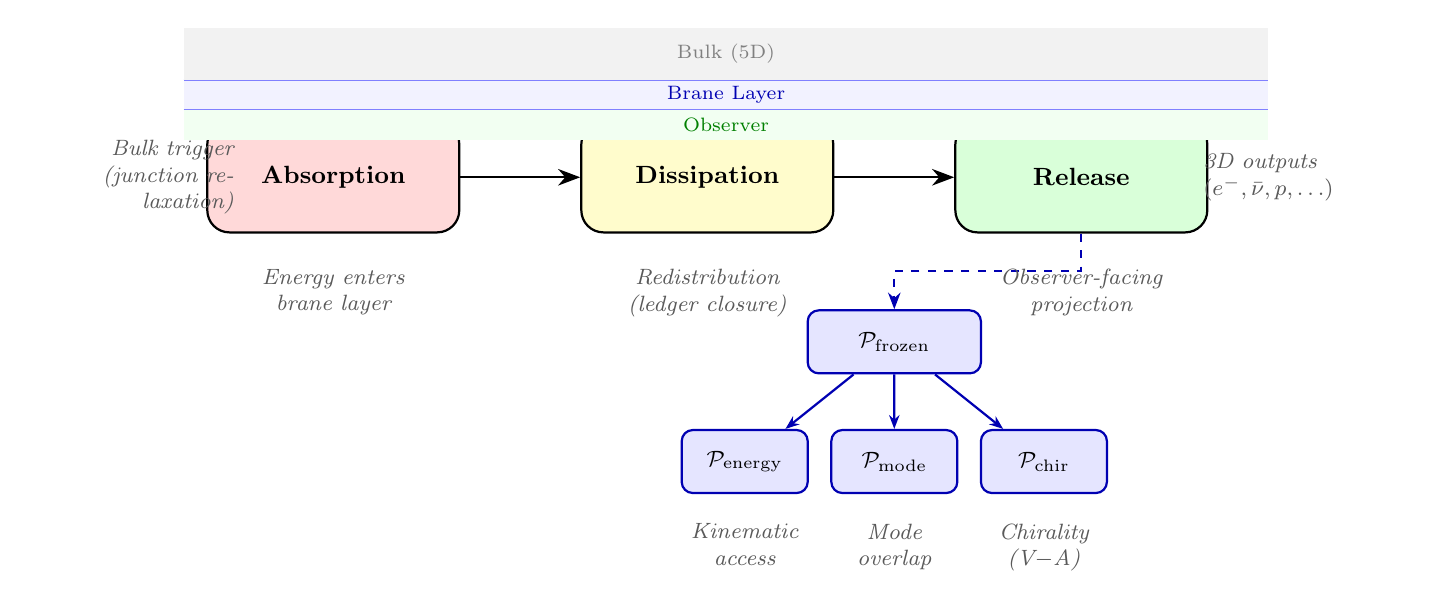
\begin{tikzpicture}[
  scale=0.95,
  stage/.style={
    rectangle, rounded corners=8pt, minimum width=3.2cm, minimum height=1.4cm,
    draw=black, thick, font=\small\bfseries
  },
  operator/.style={
    rectangle, rounded corners=4pt, minimum width=2.2cm, minimum height=0.8cm,
    draw=blue!70!black, thick, fill=blue!10, font=\footnotesize
  },
  arrow/.style={-{Stealth[length=8pt]}, thick, black},
  label/.style={font=\footnotesize\itshape, text=gray!70!black}
]

% === Stage boxes ===
\node[stage, fill=red!15] (abs) at (0,0) {Absorption};
\node[stage, fill=yellow!20] (dis) at (5,0) {Dissipation};
\node[stage, fill=green!15] (rel) at (10,0) {Release};

% === Main flow arrows ===
\draw[arrow] (abs) -- (dis);
\draw[arrow] (dis) -- (rel);

% === Projection operator box ===
\node[operator] (pfrozen) at (7.5, -2.2) {$\mathcal{P}_{\mathrm{frozen}}$};

% === Sub-operators ===
\node[operator, minimum width=1.6cm] (penergy) at (5.5, -3.8) {$\mathcal{P}_{\mathrm{energy}}$};
\node[operator, minimum width=1.6cm] (pmode) at (7.5, -3.8) {$\mathcal{P}_{\mathrm{mode}}$};
\node[operator, minimum width=1.6cm] (pchir) at (9.5, -3.8) {$\mathcal{P}_{\mathrm{chir}}$};

% === Operator decomposition ===
\draw[-{Stealth[length=5pt]}, thick, blue!70!black] (pfrozen) -- (penergy);
\draw[-{Stealth[length=5pt]}, thick, blue!70!black] (pfrozen) -- (pmode);
\draw[-{Stealth[length=5pt]}, thick, blue!70!black] (pfrozen) -- (pchir);

% === Hook from Release to P_frozen ===
\draw[-{Stealth[length=6pt]}, thick, dashed, blue!70!black]
  (rel.south) -- ++(0,-0.5) -| (pfrozen.north);

% === Input/output labels ===
\node[label, anchor=east, text width=2.5cm, align=right] at (-1.2, 0) {Bulk trigger\\(junction relaxation)};
\node[label, anchor=west, text width=2.5cm, align=left] at (11.5, 0) {3D outputs\\$(e^-, \bar\nu, p, \ldots)$};

% === Stage descriptions ===
\node[label, anchor=north, text width=3cm, align=center] at (0, -1.1)
  {Energy enters\\brane layer};
\node[label, anchor=north, text width=3cm, align=center] at (5, -1.1)
  {Redistribution\\(ledger closure)};
\node[label, anchor=north, text width=3cm, align=center] at (10, -1.1)
  {Observer-facing\\projection};

% === Operator labels ===
\node[label, anchor=north, text width=1.5cm, align=center] at (5.5, -4.5) {Kinematic\\access};
\node[label, anchor=north, text width=1.5cm, align=center] at (7.5, -4.5) {Mode\\overlap};
\node[label, anchor=north, text width=1.5cm, align=center] at (9.5, -4.5) {Chirality\\(V$-$A)};

% === Brane layer indicator ===
\fill[blue!5] (-2, 0.9) rectangle (12.5, 1.3);
\draw[thick, blue!50] (-2, 0.9) -- (12.5, 0.9);
\draw[thick, blue!50] (-2, 1.3) -- (12.5, 1.3);
\node[font=\scriptsize, blue!70!black] at (5.25, 1.1) {Brane Layer};

% === Bulk indicator ===
\fill[gray!10] (-2, 1.3) rectangle (12.5, 2.0);
\node[font=\scriptsize, gray] at (5.25, 1.65) {Bulk (5D)};

% === Observer indicator ===
\fill[green!5] (-2, 0.5) rectangle (12.5, 0.9);
\node[font=\scriptsize, green!50!black] at (5.25, 0.7) {Observer};

\end{tikzpicture}

\caption{Unified weak decay pipeline: Absorption $\to$ Dissipation $\to$
Release. The frozen projection operator $\mathcal{P}_{\mathrm{frozen}}$
filters outputs via energy, mode-matching, and chirality constraints.}
\label{fig:pipeline}
\end{figure}

% ==============================================================================
\section{Ontology Map and Dependency Graph}
\label{sec:ontology}
% ==============================================================================

The particles addressed in the Weak Sector program fall into distinct
ontological categories based on their 5D profiles.

\subsection{Ontological Classification}

\begin{table}[ht]
\centering
\caption{Particle ontologies in the EDC Weak Sector}
\label{tab:ontology}
\begin{tabular}{lllll}
\toprule
\textbf{Particle} & \textbf{Ontology} & \textbf{5D Profile} & \textbf{Companion} & \textbf{Tag} \\
\midrule
Neutron & Bulk-core junction & Extended into bulk & N & [P] \\
Proton & Bulk-core junction (stable) & Steiner $120^\circ$ & Paper 3 & [P] \\
\midrule
Electron & Brane defect (observer-facing) & Localized at $y \approx 0$ & L & [P] \\
Muon & Brane-dominant (fundamental) & Localized, mode $n_\mu$ & M & [P] \\
Tau & Brane-dominant (higher mode) & Localized, mode $n_\tau$ & T & [P] \\
\midrule
Neutrino & Edge mode (interfacial) & At bulk--brane interface & V & [P] \\
\midrule
Pion & Brane-dominant (composite) & Bound state on brane & P & [P] \\
\bottomrule
\end{tabular}
\end{table}

\subsection{Ontology Descriptions}

\textbf{Bulk-core junction (Neutron/Proton).}
The nucleons are modeled as Y-junction configurations with significant
amplitude extending into the fifth dimension. The proton sits at the Steiner
minimum (stable); the neutron has oscillation modes leading to instability
(decay to proton via junction relaxation).

\textbf{Brane-dominant excitations (Electron, Muon, Tau).}
Charged leptons are brane-layer excitations localized near the observer-facing
boundary. They differ by mode index: $n_e < n_\mu < n_\tau$, with higher modes
corresponding to higher masses \tagP{}/\tagOpen{}.

\textbf{Edge mode (Neutrino).}
The neutrino resides at the bulk--brane interface---neither fully bulk nor
fully brane-bound. Its weak interaction arises from suppressed coupling across
this interface, not from ``escape into the bulk.''

\textbf{Brane-dominant composite (Pion).}
The pion is a brane-layer bound state of constituent quarks, with energy
predominantly localized on the brane. It provides the first hadron $\to$ lepton
injection test of the pipeline.

\subsection{Dependency Graph}

Figure~\ref{fig:ontology} shows the ontological categories and document
dependencies.

\begin{figure}[ht]
\centering
% ==============================================================================
% Figure: Ontology Map and Document Dependencies
% Bulk-core vs brane-dominant vs edge mode vs composite
% ==============================================================================

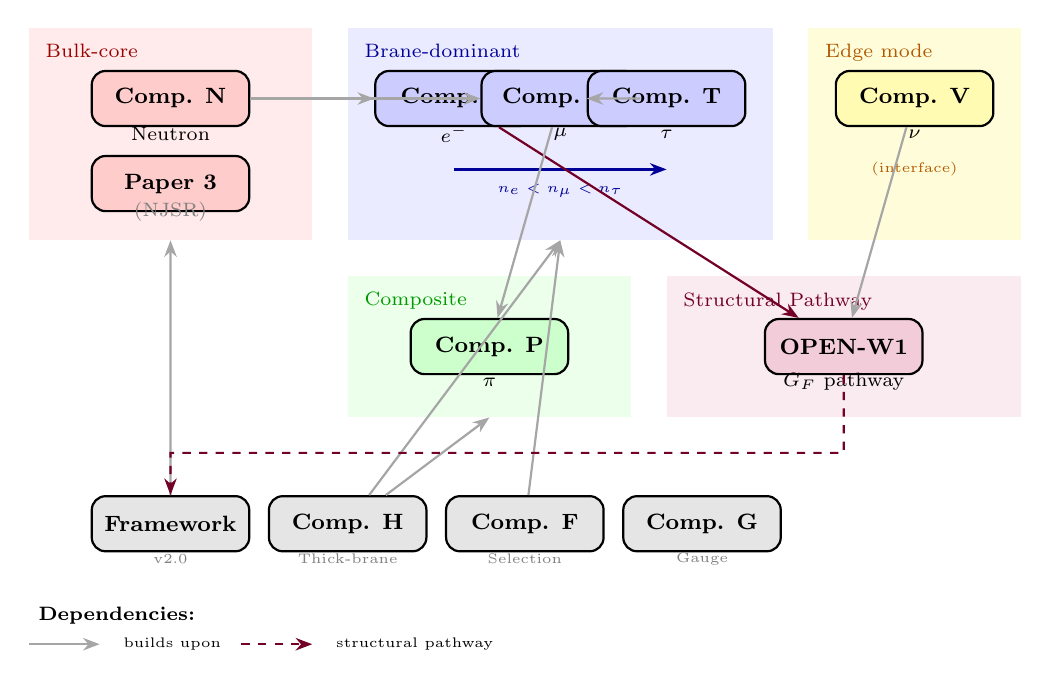
\begin{tikzpicture}[
  scale=0.9,
  doc/.style={
    rectangle, rounded corners=5pt, minimum width=2.0cm, minimum height=0.7cm,
    draw=black, thick, font=\footnotesize\bfseries
  },
  category/.style={
    rectangle, rounded corners=8pt, draw=gray, dashed, thick,
    inner sep=10pt
  },
  arrow/.style={-{Stealth[length=6pt]}, thick, gray!70},
  particle/.style={circle, draw, thick, minimum size=0.6cm, font=\footnotesize\bfseries}
]

% === Background regions ===
% Bulk region
\fill[red!8] (-5.5, 2.5) rectangle (-1.5, 5.5);
\node[font=\scriptsize, red!60!black, anchor=north west] at (-5.4, 5.4)
  {Bulk-core};

% Brane-dominant region
\fill[blue!8] (-1, 2.5) rectangle (5, 5.5);
\node[font=\scriptsize, blue!60!black, anchor=north west] at (-0.9, 5.4)
  {Brane-dominant};

% Edge mode region
\fill[yellow!15] (5.5, 2.5) rectangle (8.5, 5.5);
\node[font=\scriptsize, orange!70!black, anchor=north west] at (5.6, 5.4)
  {Edge mode};

% Composite region
\fill[green!8] (-1, 0) rectangle (3, 2);
\node[font=\scriptsize, green!60!black, anchor=north west] at (-0.9, 1.9)
  {Composite};

% OPEN pathway region
\fill[purple!8] (3.5, 0) rectangle (8.5, 2);
\node[font=\scriptsize, purple!60!black, anchor=north west] at (3.6, 1.9)
  {Structural Pathway};

% === Document nodes ===
% Bulk-core
\node[doc, fill=red!20] (N) at (-3.5, 4.5) {Comp. N};
\node[doc, fill=red!20] (P3) at (-3.5, 3.3) {Paper 3};
\node[font=\scriptsize] at (-3.5, 4.0) {Neutron};
\node[font=\scriptsize, gray] at (-3.5, 2.9) {(NJSR)};

% Brane-dominant
\node[doc, fill=blue!20] (L) at (0.5, 4.5) {Comp. L};
\node[doc, fill=blue!20] (M) at (2.0, 4.5) {Comp. M};
\node[doc, fill=blue!20] (T) at (3.5, 4.5) {Comp. T};
\node[font=\scriptsize] at (0.5, 4.0) {$e^-$};
\node[font=\scriptsize] at (2.0, 4.0) {$\mu$};
\node[font=\scriptsize] at (3.5, 4.0) {$\tau$};

% Mode index arrow
\draw[arrow, blue!60!black] (0.5, 3.5) -- (3.5, 3.5);
\node[font=\tiny, blue!60!black] at (2.0, 3.2) {$n_e < n_\mu < n_\tau$};

% Edge mode
\node[doc, fill=yellow!30] (V) at (7.0, 4.5) {Comp. V};
\node[font=\scriptsize] at (7.0, 4.0) {$\nu$};
\node[font=\tiny, orange!70!black] at (7.0, 3.5) {(interface)};

% Composite
\node[doc, fill=green!20] (P) at (1.0, 1.0) {Comp. P};
\node[font=\scriptsize] at (1.0, 0.5) {$\pi$};

% OPEN pathway
\node[doc, fill=purple!20] (W1) at (6.0, 1.0) {OPEN-W1};
\node[font=\scriptsize] at (6.0, 0.5) {$G_F$ pathway};

% === Foundation documents ===
\node[doc, fill=gray!20] (Fw) at (-3.5, -1.5) {Framework};
\node[doc, fill=gray!20] (H) at (-1.0, -1.5) {Comp. H};
\node[doc, fill=gray!20] (F) at (1.5, -1.5) {Comp. F};
\node[doc, fill=gray!20] (G) at (4.0, -1.5) {Comp. G};
\node[font=\tiny, gray] at (-3.5, -2.0) {v2.0};
\node[font=\tiny, gray] at (-1.0, -2.0) {Thick-brane};
\node[font=\tiny, gray] at (1.5, -2.0) {Selection};
\node[font=\tiny, gray] at (4.0, -2.0) {Gauge};

% === Dependency arrows ===
% From foundations up
\draw[arrow] (Fw) -- (-3.5, 2.5);
\draw[arrow] (H) -- (1.0, 0);
\draw[arrow] (H) -- (2.0, 2.5);
\draw[arrow] (F) -- (2.0, 2.5);

% N to leptons
\draw[arrow] (N) -- (L);
\draw[arrow] (N) -- (M);

% M to T
\draw[arrow] (M) -- (T);

% V connection
\draw[arrow] (V) -- (W1);
\draw[arrow, purple!60!black] (L) -- (W1);

% P connection
\draw[arrow] (M) -- (P);

% Pipeline connection
\draw[arrow, dashed, purple!60!black] (W1) -- (6.0, -0.5) -- (-3.5, -0.5) -- (Fw);

% === Legend ===
\node[font=\scriptsize\bfseries, anchor=west] at (-5.5, -2.8) {Dependencies:};
\draw[arrow] (-5.5, -3.2) -- (-4.5, -3.2);
\node[font=\tiny, anchor=west] at (-4.3, -3.2) {builds upon};
\draw[arrow, dashed, purple!60!black] (-2.5, -3.2) -- (-1.5, -3.2);
\node[font=\tiny, anchor=west] at (-1.3, -3.2) {structural pathway};

\end{tikzpicture}

\caption{Ontology map and document dependencies. Bulk-core junctions (N)
differ from brane-dominant excitations (L, M, T) and composites (P). The
neutrino (V) is an edge mode. OPEN-W1 provides the $G_F$ structural pathway.}
\label{fig:ontology}
\end{figure}

% ==============================================================================
\section{Case Studies: Module Summaries}
\label{sec:cases}
% ==============================================================================

Each companion document addresses a specific particle within the unified
pipeline. We summarize each using a consistent template.

% ------------------------------------------------------------------------------
\subsection{Neutron Decay (Companion N)}
\label{subsec:neutron}

\textbf{DOI:} 10.5281/zenodo.18315110

\textbf{Baselines [BL]:}
\begin{itemize}[nosep]
  \item $\tau_n = 878.4 \pm 0.5$ s (PDG 2024)
  \item $Q_\beta = 1.293$ MeV
  \item Decay: $n \to p + e^- + \bar\nu_e$
\end{itemize}

\textbf{Mechanism [P]/[Dc]:}
\begin{itemize}[nosep]
  \item Neutron = bulk-core Y-junction with oscillation modes
  \item Instability from junction relaxation (Steiner deviation)
  \item Nuclear stabilization via modified boundary conditions in nuclei
\end{itemize}

\textbf{Closure Targets [OPEN]:}
\begin{itemize}[nosep]
  \item Derive $\tau_n$ from junction geometry
  \item Quantify nuclear stabilization mechanism
  \item Connect to $G_F$ via OPEN-W1 pathway
\end{itemize}

\textbf{Pipeline connection.}
The neutron junction relaxation provides the \emph{bulk trigger} (Absorption).
Energy dissipates through brane-layer modes and releases as $p + e^- + \bar\nu_e$
via the frozen projection operator.

% ------------------------------------------------------------------------------
\subsection{Muon Decay (Companion M)}
\label{subsec:muon}

\textbf{DOI:} 10.5281/zenodo.18319888

\textbf{Baselines [BL]:}
\begin{itemize}[nosep]
  \item $\tau_\mu = 2.197 \times 10^{-6}$ s
  \item $m_\mu = 105.66$ MeV
  \item Decay: $\mu^- \to e^- + \bar\nu_e + \nu_\mu$
\end{itemize}

\textbf{Mechanism [P]/[Dc]:}
\begin{itemize}[nosep]
  \item Muon = brane-dominant excitation, mode index $n_\mu > n_e$
  \item Decay via de-excitation within brane layer
  \item Same pipeline structure as neutron (validates universality)
\end{itemize}

\textbf{Closure Targets [OPEN]:}
\begin{itemize}[nosep]
  \item Derive $\tau_\mu$ from mode-spectrum analysis
  \item Quantify mode index $n_\mu$ from brane geometry
  \item Derive mass ratio $m_\mu/m_e \approx 207$ from mode structure
\end{itemize}

\textbf{Pipeline connection.}
The muon provides a \emph{clean test case} with no hadronic complications.
The higher mode ($n_\mu$) de-excites to lower mode ($n_e$) plus two neutrinos,
conserving all ledger quantities.

% ------------------------------------------------------------------------------
\subsection{Tau Decay (Companion T)}
\label{subsec:tau}

\textbf{DOI:} 10.5281/zenodo.18319900

\textbf{Baselines [BL]:}
\begin{itemize}[nosep]
  \item $\tau_\tau = 2.903 \times 10^{-13}$ s
  \item $m_\tau = 1776.86$ MeV
  \item BR($\tau \to e$) $\approx$ BR($\tau \to \mu$) $\approx 17.8\%$
\end{itemize}

\textbf{Mechanism [P]/[Dc]:}
\begin{itemize}[nosep]
  \item Tau = brane-dominant excitation, mode index $n_\tau > n_\mu > n_e$
  \item Mode-spectrum overlap explains near-equal BR to $e$ and $\mu$
  \item Pipeline generalizes without modification
\end{itemize}

\textbf{Closure Targets [OPEN]:}
\begin{itemize}[nosep]
  \item Derive $\tau_\tau$ from first principles
  \item Explain BR equality quantitatively
  \item Address hadronic tau decays
\end{itemize}

\textbf{Pipeline connection.}
The tau provides a \emph{mode-spectrum test}: if muon and tau share the same
ontology, the pipeline should generalize. The near-equal branching ratios
to $e$ and $\mu$ suggest similar mode-spectrum overlaps \tagP{}/\tagOpen{}.

% ------------------------------------------------------------------------------
\subsection{Pion Decay (Companion P)}
\label{subsec:pion}

\textbf{DOI:} 10.5281/zenodo.18319913

\textbf{Baselines [BL]:}
\begin{itemize}[nosep]
  \item $\tau_{\pi^\pm} = 2.6 \times 10^{-8}$ s
  \item $m_\pi = 139.57$ MeV
  \item BR($\pi \to \mu\nu$)/BR($\pi \to e\nu$) $\approx 8000$ (helicity suppression)
\end{itemize}

\textbf{Mechanism [P]/[Dc]:}
\begin{itemize}[nosep]
  \item Pion = brane-dominant composite (bound state)
  \item Helicity suppression from $\mathcal{P}_{\mathrm{chir}}$ selection
  \item First hadron $\to$ lepton injection test
\end{itemize}

\textbf{Closure Targets [OPEN]:}
\begin{itemize}[nosep]
  \item Derive $m_\pi$ from 5D binding
  \item Derive helicity suppression ($m_\ell^2$ scaling) from BC
  \item Validate junction-pair micro-ontology
\end{itemize}

\textbf{Pipeline connection.}
The pion provides the \emph{hadron $\to$ lepton bridge}: a composite initial
state decaying to leptonic final states via the same pipeline. The $m_\ell^2$
helicity suppression is treated as \tagBL{}; its derivation from EDC BC
remains \tagOpen{}.

% ------------------------------------------------------------------------------
\subsection{Electron as Brane Defect (Companion L)}
\label{subsec:electron}

\textbf{DOI:} 10.5281/zenodo.18321357

\textbf{Baselines [BL]:}
\begin{itemize}[nosep]
  \item $m_e = 0.511$ MeV (stable)
  \item Charge $q = -1$, spin $1/2$
  \item Kinematic access: $Q_\beta - m_e = +0.782$ MeV (allowed in $\beta^-$)
\end{itemize}

\textbf{Mechanism [P]/[Dc]:}
\begin{itemize}[nosep]
  \item Electron = stable topological defect on observer-facing layer
  \item Localized at $y \approx 0$ (maximal observer coupling)
  \item Selected by frozen projection: kinematic + ledger + chirality
\end{itemize}

\textbf{Closure Targets [OPEN]:}
\begin{itemize}[nosep]
  \item Derive $m_e$ from defect structure
  \item Explain mass hierarchy $m_\mu/m_e \approx 207$
  \item Derive electron spin from 5D topology
\end{itemize}

\textbf{Pipeline connection.}
The electron is the \emph{primary allowed output} of neutron $\beta^-$ decay:
kinematically accessible ($Q > m_e$), ledger-closing (carries charge and
lepton number), and chirality-selected (left-handed).

% ------------------------------------------------------------------------------
\subsection{Neutrino as Edge Mode (Companion V)}
\label{subsec:neutrino}

\textbf{DOI:} 10.5281/zenodo.18321383

\textbf{Baselines [BL]:}
\begin{itemize}[nosep]
  \item Masses: $m_\nu < 0.8$ eV (cosmological bound)
  \item Helicity: left-handed $\nu$, right-handed $\bar\nu$ (V$-$A)
  \item Three flavors: $\nu_e$, $\nu_\mu$, $\nu_\tau$
\end{itemize}

\textbf{Mechanism [P]/[Dc]:}
\begin{itemize}[nosep]
  \item Neutrino = edge mode at bulk--brane interface
  \item Weak interaction from \emph{suppressed leakage}, not ``bulk escape''
  \item Chirality filter $\mathcal{P}_{\mathrm{chir}}$ selects helicity
\end{itemize}

\textbf{Closure Targets [OPEN]:}
\begin{itemize}[nosep]
  \item Derive neutrino masses from interface structure
  \item Explain three-flavor structure
  \item Address Dirac vs.\ Majorana nature
\end{itemize}

\textbf{Pipeline connection.}
The neutrino is the \emph{ledger-closure partner}: it carries away spin,
momentum, and lepton number without appearing as a charged output. Its
``invisibility'' arises from suppressed coupling across the interface, not
from being ``elsewhere.''

% ==============================================================================
\section{Structural Pathway to \texorpdfstring{$G_F$}{GF}}
\label{sec:GF}
% ==============================================================================

This section promotes the structural derivation from OPEN-W1
(DOI: 10.5281/zenodo.18321396) to the journal presentation.

\subsection{The Structural Scaling}

Integrating out a brane-layer mediator $\phi$ at tree level yields:
\begin{equation}
  \boxed{
    \mathcal{L}_{\mathrm{eff}} = -\frac{g_5^2}{2 m_\phi^2} \,
    \mathcal{O}_{\mathrm{overlap}} \, J(x) J(x)
  }
  \label{eq:L_eff_main}
\end{equation}
where $J(x)$ is the source current from the bulk trigger and
$\mathcal{O}_{\mathrm{overlap}}$ encodes wavefunction overlaps.

\begin{tcolorbox}[edcCornerstone, title={Canonical Physical Interpretation [Dc]}]
Equation~\eqref{eq:L_eff_main} is \textbf{not} a fundamental ``weak vertex'';
it is the low-energy residue of a 5D bulk$\to$brane transfer process. The
source $J(x)$ represents bulk-facing pumping into the brane layer via the
mediator $\phi$ at $y = -\delta/2$; integrating out $\phi$ compresses that
transfer into an effective local contact $JJ$ term. The apparent smallness
of the coupling is therefore a \textbf{geometric suppression}---set by the
mediator gap $m_\phi$, mode-profile overlap, and boundary/projection factors
---rather than a tunable parameter.
\end{tcolorbox}

\subsection{EDC Structural Analog}

Comparing with the Fermi form, we define \tagDef{}:
\begin{equation}
  \boxed{
    G_{\mathrm{EDC}} \sim \frac{g_{\mathrm{eff}}^2}{m_\phi^2}
  }
  \label{eq:G_EDC_main}
\end{equation}
where the effective coupling decomposes as:
\begin{equation}
  \boxed{
    g_{\mathrm{eff}} = g_5 \times \mathcal{O}_{\mathrm{overlap}}
    \times \mathcal{O}_{\mathrm{BC}}
  }
  \label{eq:geff_main}
\end{equation}

\textbf{Factor decomposition.}
\begin{itemize}[nosep]
  \item $g_5$: fundamental 5D coupling scale \tagOpen{}
  \item $\mathcal{O}_{\mathrm{overlap}}$: wavefunction overlap integral
        $\sim \int dy \, f_a f_b f_\phi$ \tagOpen{}
  \item $\mathcal{O}_{\mathrm{BC}} = \mathcal{O}(\mathcal{P}_{\mathrm{frozen}},
        \mathcal{P}_{\mathrm{chir}})$: boundary-condition/projection factor
        \tagP{}/\tagDc{}
\end{itemize}

The chirality filter $\mathcal{P}_{\mathrm{chir}}$ (Companion V) enters
$\mathcal{O}_{\mathrm{BC}}$, producing V$-$A structure as an \emph{output}
of boundary conditions.

\subsection{Dimensional Analysis}

In natural units ($\hbar = c = 1$):
\begin{equation}
  [G_{\mathrm{EDC}}] = \frac{[g_{\mathrm{eff}}]^2}{[m_\phi]^2}
  = \frac{[E]^{-1}}{[E]^2} = [E]^{-2} \quad \checkmark
  \label{eq:dim_main}
\end{equation}
This matches the required dimension of a four-fermion coupling constant.

\subsection{Closure Checklist}

A complete derivation of $G_F$ (not just its structure) requires:
\begin{enumerate}[nosep]
  \item \textbf{Mode profiles}: solve thick-brane BVP for $f_a$, $f_b$, $f_\phi$
        \tagOpen{}
  \item \textbf{KK spectrum}: derive $m_\phi$ from $\xi$-sector geometry
        \tagOpen{}
  \item \textbf{BC operator evaluation}: compute
        $\mathcal{O}(\mathcal{P}_{\mathrm{frozen}}, \mathcal{P}_{\mathrm{chir}})$
        \tagOpen{}
  \item \textbf{Coupling origin}: derive $g_5$ from 5D action normalization
        \tagOpen{}
\end{enumerate}

\begin{tcolorbox}[edcWarning, title={No-Fit Statement}]
\textbf{No parameter in this derivation is tuned to match the PDG value
$G_F = 1.166 \times 10^{-5}~\mathrm{GeV}^{-2}$.} That value is a \tagBL{}
benchmark. Any future numerical derivation must obtain $G_F$ from geometric
quantities without fitting to weak observables.
\end{tcolorbox}

% ==============================================================================
\section{Falsifiability and Non-Overclaim Canon}
\label{sec:falsifiability}
% ==============================================================================

\subsection{Falsifiability Handles}

The EDC Weak Sector makes specific structural predictions that can be tested:

\begin{enumerate}
  \item \textbf{Pipeline universality}: If any weak decay cannot be mapped to
        Absorption $\to$ Dissipation $\to$ Release, the framework fails.

  \item \textbf{Ontology consistency}: If a bulk-core particle behaves as
        brane-dominant (or vice versa), the ontology classification fails.

  \item \textbf{Selection rule validity}: If forbidden channels (e.g.,
        $\mu^- \to e^- + \gamma$ at tree level) are observed at rates
        inconsistent with suppression, the $\mathcal{P}_{\mathrm{frozen}}$
        structure fails.

  \item \textbf{Chirality filter}: If right-handed $W$ bosons or V$+$A currents
        are discovered with SM-like coupling, $\mathcal{P}_{\mathrm{chir}}$
        fails.

  \item \textbf{Helicity in decays}: If neutrinos are detected with wrong-sign
        helicity at appreciable rates, the edge-mode hypothesis fails.

  \item \textbf{Ledger closure}: If energy/momentum accounting in weak decays
        shows systematic deviations beyond neutrino mass effects, the
        bulk--brane conservation mechanism fails.

  \item \textbf{Nuclear stabilization}: If free neutron decay rate varies with
        environment in ways inconsistent with BC modification, the junction
        model fails.

  \item \textbf{Geometric suppression}: If $G_F$ shows energy dependence
        inconsistent with mediator-exchange structure, the structural pathway
        fails.
\end{enumerate}

\subsection{Non-Overclaim Canon}

\begin{tcolorbox}[edcGuardrail, title={What We Do NOT Claim}]
The EDC Weak Sector does \textbf{NOT} claim:
\begin{itemize}[nosep]
  \item Numerical derivation of particle masses
  \item Numerical derivation of lifetimes
  \item Derivation of branching ratios beyond selection-rule constraints
  \item Explanation of CP violation
  \item Resolution of the strong CP problem
  \item Complete unification with gravity
  \item Full Standard Model derivation
\end{itemize}
All numerical values are either \tagBL{} (empirical) or \tagOpen{} (pending).
\end{tcolorbox}

% ==============================================================================
\section{Roadmap of OPEN Problems}
\label{sec:roadmap}
% ==============================================================================

\subsection{Grouped OPEN Items}

\begin{longtable}{lp{5cm}p{5cm}}
\caption{Consolidated OPEN problems by category}
\label{tab:open} \\
\toprule
\textbf{Category} & \textbf{Problem} & \textbf{Candidate Approach} \\
\midrule
\endfirsthead
\toprule
\textbf{Category} & \textbf{Problem} & \textbf{Candidate Approach} \\
\midrule
\endhead
\multirow{3}{*}{Geometry/Modes}
  & Fermion mode profiles $f_a$, $f_b$ & Thick-brane BVP solution \\
  & Mediator profile $f_\phi$ & KK reduction in frozen regime \\
  & Brane thickness $\delta$ & Framework v2.0 + $\sigma$ relationship \\
\midrule
\multirow{2}{*}{BC Operators}
  & $\mathcal{P}_{\mathrm{frozen}}$ explicit form & Companion H + F integration \\
  & $\mathcal{P}_{\mathrm{chir}}$ derivation from BC & Companion V + spinor BC analysis \\
\midrule
\multirow{2}{*}{Mediator Spectrum}
  & $m_\phi$ from $\xi$-geometry & KK analysis of throat modes \\
  & Coupling $g_5$ normalization & 5D action principle \\
\midrule
\multirow{2}{*}{Ledger Partition}
  & Energy split in three-body decays & Phase-space + mode overlap \\
  & Neutrino spectrum shape & Interface mode structure \\
\midrule
\multirow{2}{*}{Compositeness}
  & Pion micro-ontology & Junction-pair hypothesis \\
  & Quark confinement in 5D & Open (beyond current scope) \\
\bottomrule
\end{longtable}

\subsection{Priority: Next Hard Step}

The highest-impact next step is:
\begin{tcolorbox}[edcCornerstone, title={Priority Closure Target}]
\textbf{Derive mode profiles + KK spectrum + BC operator evaluation.}

This would:
\begin{enumerate}[nosep]
  \item Provide explicit $\mathcal{O}_{\mathrm{overlap}}$ value
  \item Determine $m_\phi$ from geometry
  \item Enable numerical check of $G_{\mathrm{EDC}}$ against $G_F$
  \item Test whether ``geometric suppression'' quantitatively works
\end{enumerate}

\textbf{Required inputs:} Thick-brane BVP (Companion H), frozen regime
parameters (Framework v2.0), chirality BC (Companion V).

\textbf{Status:} \tagOpen{}
\end{tcolorbox}

% ==============================================================================
\section{Conclusion}
\label{sec:conclusion}
% ==============================================================================

The EDC Weak Sector program demonstrates that a single mechanistic
framework---based on thick-brane microphysics with a unified
Absorption $\to$ Dissipation $\to$ Release pipeline---can accommodate weak
decays across diverse particle ontologies:

\begin{itemize}[nosep]
  \item \textbf{Bulk-core junctions}: neutron (unstable), proton (stable)
  \item \textbf{Brane-dominant excitations}: electron, muon, tau
  \item \textbf{Edge modes}: neutrino (interfacial, suppressed leakage)
  \item \textbf{Composites}: pion (brane-layer bound state)
\end{itemize}

The structural pathway to $G_F$---showing $G_{\mathrm{EDC}} \sim
g_{\mathrm{eff}}^2/m_\phi^2$ as geometric suppression---provides a
falsifiable mechanism without numerical fitting. The chirality filter
$\mathcal{P}_{\mathrm{chir}}$ produces V$-$A structure as an output of
boundary conditions.

\textbf{What remains.}
Numerical closure requires deriving mode profiles, KK spectrum, and BC
operators from the thick-brane geometry. These are explicitly catalogued
as \tagOpen{} items with clear closure pathways. The framework is designed
to either succeed quantitatively or fail falsifiably---there is no room for
post-hoc adjustment.

\vspace{1em}
\begin{center}
\rule{0.5\textwidth}{0.4pt}
\end{center}
\vspace{0.5em}

\noindent\textit{Document version: Paper 3J (Journal Synthesis)}\\
\textit{Generated: January 2026}\\
\textit{This paper provides the primary reading path for the EDC Weak Program;
the Overview remains an internal registry/index. All companions remain archival
modules with DOIs.}

% ==============================================================================
\end{document}
% ==============================================================================
